\documentclass{article}

\usepackage{amsmath}
\usepackage{amssymb}
\usepackage{amsthm}
\usepackage[hidelinks]{hyperref}
\usepackage{xcolor}
\usepackage{bbm}
\usepackage{arydshln}
\usepackage{mathtools}
\usepackage{pdfpages}

%\usepackage[includefoot, a4paper, total={7in, 9in}]{geometry}
\usepackage{geometry}
 \geometry{
 a4paper,
 total={170mm,257mm},
 left=20mm,
 top=20mm,
 }
\usepackage{blindtext}
\usepackage{lastpage}
\usepackage{fancyhdr}
\pagestyle{fancy}
\fancyhf{} 
\fancyfoot[R]{Page \thepage}

\newtheorem{definition}{Definition}
\newtheorem{theorem}{Theorem}
\newtheorem{lemma}{Lemma}
\newtheorem{ex}{Example}
\newtheorem{rk}{Remark}
\newtheorem{prop}{Proposition}

\newcommand\eqd{\stackrel{\mathclap{\normalfont\mbox{d}}}{=}}

\begin{document}

    \section{Stochastic Differential Equation}

Consider the following stochastic differential equation (SDE)

\begin{equation} \label{sde}
dX_t = b(t,X_t)dt + \sigma(t,X_t)dW_t,
\end{equation}
where $b$ is drift term, $\sigma$ is the dispersion, and $W_t$ is a one-dimensional Brownian motion. Here we consider functions $b$ and $\sigma$ to be Borel-measurable functions from $\mathbb{R}_+\times\mathbb{R}$ to $\mathbb{R}$. The SDE \eqref{sde} can be equivalently written in the following integral form:

\begin{equation*}
X_t = x + \int_0^t b(s,X_s)ds + \int^t_0 \sigma(s,X_s)dW_s.
\end{equation*}

\subsection{Strong Solution}
In this part, we are interested in the conditions under which the SDE \eqref{sde} has strong existence and strong uniqueness. Recall that for an ordinary differential equation (ODE), shown as below:

\begin{equation} \label{ode}
x'(t) = b(t,x(t)),
\end{equation}

the Picard-Lindelof/Cauchy-Lipschitz theorem states that if the function $b$ is Lipschitz with respect to the state variable, then there exists a solution to the ODE \eqref{ode}. This is to say that there exists a constant $K$ such that $|b(t,x)-b(t,y)|\leq K|x-y|$. For uniqueness of the solution, locally Lipschitz condition is enough. This is to say that for all $R>0$, there exists a constant $K_R$, depending on $R$, such that $|b(t,x)-b(t,y)|\leq K_R|x-y|$ for all $x,y\in[-R,R]$.

We can define similar conditions to show the strong existence and strong uniqueness for the SDE \eqref{sde}. We start by introducing the Gronwall inequality, which will be useful for proving the uniqueness results.
 
\begin{lemma} \label{lemma:gronwall} \textcolor{red}{(Gronwall Inequality)}

Suppose that the measurable function $f:[0,\infty)\rightarrow\mathbb{R}$ satisfies

\begin{equation*}
0\leq f(t)\leq a+b\int^t_0 f(s)ds,
\end{equation*}
for some $a,b\in\mathbb{R}$. Then, 

\begin{equation*}
f(t)\leq ae^{bt}.
\end{equation*}

\end{lemma}

The proof for this Lemma is omitted, and we introduce the uniqueness result here.

\begin{theorem} \label{thm:strong_uniqueness} \textcolor{red}{(Strong Uniqueness)}

If for all $R>0$, there exists a constant $C_R$ such that for all $t\geq0$ and for all $x,y\in[-R,R]$, the following conditions hold for the functions $b$ and $\sigma$ in the SDE \eqref{sde}

\begin{equation*}
\begin{aligned}
&|b(t,x)-b(t,y)|\leq C_R|x-y|\\
&|\sigma(t,x)-\sigma(t,y)|\leq C_R|x-y|,
\end{aligned}
\end{equation*}
then strong uniqueness holds for the SDE \eqref{sde}.

\end{theorem}

\begin{proof}
Let $X$ and $\tilde{X}$ be two strong solutions to the SDE \eqref{sde}. Define $Y_t:=X_t-\tilde{X}_t$. We would like to compute $\mathbb{E}[Y_t^2]$. From Ito's formula, we have:

\begin{equation}\label{proof:uniqueness}
\begin{aligned}
Y_t^2 &= Y_0^2 + 2\int^t_0 Y_sdY_s + \int^t_0 d\langle Y \rangle_s\\
&=2\int^t_0 Y_s(b(s,X_s)-b(s,\tilde{X}_s))ds + 2\int^t_0 Y_s(\sigma(s,X_s)-\sigma(s,\tilde{X}_s))dW_s + \int^t_0 (\sigma(s,X_s)-\sigma(s,\tilde{X}_s))^2ds.
\end{aligned}
\end{equation}

Now, for a fixed $R>0$, define the stopping time as follows

\begin{equation*}
\tau_R = \inf \{t \geq 0: |X_s|\geq R \quad \text{or} \quad |\tilde{X}_s|\geq R\}.
\end{equation*}

With this localization, we would like to show that the stochastic integral is a martingale. We first show that the integrand is square-integrable.

\begin{equation*}
\mathbb{E}\left[\int_0^{t\wedge\tau_R}(Y_s(\sigma(s,X_s)-\sigma(s,\tilde{X}_s)))^2ds\right]\leq C_R^2\mathbb{E}\left[\int_0^{t\wedge\tau_R}((X_s-\tilde{X}_s))^4ds\right]\leq16C_R^2R^2T<\infty.
\end{equation*}

Thus, we know $Y_s(\sigma(s,X_s)-\sigma(s,\tilde{X}_s))\in\mathcal{L}^*_W$, and the stochastic integral in \eqref{proof:uniqueness} is (locally) a martingale, which implies that its expectation is zero. Then, we (locally) bound the expectation of \eqref{proof:uniqueness} as follows:

\begin{equation*}
\begin{aligned}
0\leq\mathbb{E}[Y_{t\wedge\tau_R}^2]&=2\mathbb{E}\left[\int^{t\wedge\tau_R}_0 Y_s(b(s,X_s)-b(s,\tilde{X}_s))ds\right] + \mathbb{E}\left[\int^{t\wedge\tau_R}_0 (\sigma(s,X_s)-\sigma(s,\tilde{X}_s))^2ds\right]\\
&\leq2C_R^2\mathbb{E}\left[\int^{t\wedge\tau_R}_0 (X_s-\tilde{X}_s)^2ds\right] + C_R^2\mathbb{E}\left[\int^{t\wedge\tau_R}_0 (X_s-\tilde{X}_s)^2ds\right]\\
&=\tilde{C}\mathbb{E}\left[\int^t_0 (X_{s\wedge\tau_R}-\tilde{X}_{s\wedge\tau_R})^2ds\right]\\
&=\tilde{C}\int^t_0 \mathbb{E}\left[(X_{s\wedge\tau_R}-\tilde{X}_{s\wedge\tau_R})^2\right]ds.
\end{aligned}
\end{equation*}

Now, we are ready to use Lemma \ref{lemma:gronwall}. In particular, we have $a=0$, which implies $\mathbb{E}[Y_{t\wedge\tau_R}^2]=0$. Note $R\rightarrow\infty\Rightarrow\tau_R\rightarrow\infty\Rightarrow t\wedge\tau_R=t$. Then, by the dominated convergence theorem, we have $\mathbb{E}[Y_{t}^2]=0$. This shows that $\{X_t,0\leq t<\infty\}$ and $\{\tilde{X}_t,0\leq t<\infty\}$ are modifications of each other. Since both solutions are continuous, we know that they are indistinguishable.

\end{proof}

Next, we show the existence of the strong solution to the SDE \eqref{sde}, which asks more than locally Lipschitz for the function $b$ and $\sigma$. 

\begin{theorem} \label{thm:strong_existence} \textcolor{red}{(Strong Existence)}

Assume functions $b$ and $\sigma$ in the SDE \eqref{sde} are Lipschitz continuous and satisfy the growth condition as detailed below:

\begin{equation*}
\begin{aligned}
&|b(t,x)-b(t,y)|\leq C|x-y|\\
&|\sigma(t,x)-\sigma(t,y)|\leq C|x-y|\\
&|b(t,x)|^2+|\sigma(t,x)|^2\leq C(1+|x|^2),
\end{aligned}
\end{equation*}
for some constant $C$, then the strong existence holds for the SDE \eqref{sde}. 

Moreover, for every finite $T>0$, there exists a positive constant $\tilde{C}$, depending only on $T$ and $C$ such that

\begin{equation} \label{thm:strong_existence_integrability}
\mathbb{E}[|X_t|^2]\leq\tilde{C}(1+|x|^2)e^{\tilde{C}t}, \quad t\in[0,T].
\end{equation}

\end{theorem}

We first present the following lemma without prove.

\begin{lemma} \label{lemma:strong_existance}

Consider the following sequence of stochastic processes $\{X^{(k)}\}_{k\in\mathbb{N}}$. Starting from $X^{(0)}_t:=x$, define $X^{(k)}$ recursively as:

\begin{equation} \label{eq:iterative_process}
X^{(k+1)}_t := x + \int^t_0 b(s,X^{(k)})ds + \int^t_0 \sigma(s,X^{(k)})dW_s.
\end{equation}

Then, for each $k\in\mathbb{N}$, the process $X^{(k)}_t$ is square integrable in the following sense: for every finite $T>0$, there exists a positive constant $\tilde{C}$, depending only on $T$ and $C$ such that

\begin{equation} \label{lemma:strong_existence_integrability}
\mathbb{E}[|X_t^{(k)}|^2]\leq\tilde{C}(1+|x|^2)e^{\tilde{C}t}, \quad t\in[0,T],k\in\mathbb{N}.
\end{equation}
\end{lemma}

Now, we prove Theorem \ref{thm:strong_existence}.

\begin{proof}
The goal is to show that the sequence of stochastic processes $\{X^{(k)}\}_{k\in\mathbb{N}}$ defined recursively in \eqref{eq:iterative_process} converges to $X_t$ so that the limit of \eqref{eq:iterative_process} coincides with the SDE \eqref{sde}. Let's start with the following: 

\begin{equation*}
\begin{aligned}
\mathbb{E}\left[\max_{t\in[0,T]}|X^{(k+1)}_t-X^{(k)}_t|^2\right]=\mathbb{E}\left[\max_{t\in[0,T]}(B_t+M_t)^2\right]\leq2\mathbb{E}\left[\max_{t\in[0,T]}B_t^2\right] + 2\mathbb{E}\left[\max_{t\in[0,T]}M_t^2\right],
\end{aligned}
\end{equation*}
where

\begin{equation*}
\begin{aligned}
&B_t:=\int_0^tb(s,X^{(k)}_s)-b(s,X^{(k-1)}_s)ds\\
&M_t:=\int_0^t\sigma(s,X^{(k)}_s)-\sigma(s,X^{(k-1)}_s)dW_s.
\end{aligned}
\end{equation*}

Let's first focus on the term $B_t$. Using the Cauchy-Schwarz inequality and the Lipschitz condition on the function $b$, we have:

\begin{equation*}
\begin{aligned}
\mathbb{E}\left[\max_{t\in[0,T]}B_t^2\right]&=\mathbb{E}\left[\max_{t\in[0,T]}|\int_0^tb(s,X^{(k)}_s)-b(s,X^{(k-1)}_s)ds|^2\right]\\
&\leq\mathbb{E}\left[\max_{t\in[0,T]}t\int_0^t|b(s,X^{(k)}_s)-b(s,X^{(k-1)}_s)|^2ds\right]\\
&=\mathbb{E}\left[T\int_0^T|b(s,X^{(k)}_s)-b(s,X^{(k-1)}_s)|^2ds\right]\\
&\leq TC^2\mathbb{E}\left[\int_0^T|X^{(k)}_s-X^{(k-1)}_s|^2ds\right].
\end{aligned}
\end{equation*}

Next, we turn attention to $M_t$. From Lemma \ref{lemma:strong_existance} and the Lipschitz condition on the function $\sigma$, it is easy to show that $M_t$ is a square integrable martingale. This fact allows us to use the \textcolor{red}{BDG-inequality}, which yields the following result

\begin{equation*}
\begin{aligned}
\mathbb{E}\left[\max_{t\in[0,T]}M_t^2\right]&\leq\tilde{C}\mathbb{E}[\langle M\rangle_T]\\
&=\tilde{C}\mathbb{E}\left[\int_0^T(\sigma(s,X^{(k)}_s)-\sigma(s,X^{(k-1)}_s))^2ds\right]\\
&\leq\tilde{C}C^2\mathbb{E}\left[\int_0^T(X_s^{(k)}-X_s^{(k-1)})^2ds\right].
\end{aligned}
\end{equation*}

Combining these two results, we have:

\begin{equation} \label{pf:stong_existence}
\begin{aligned}
\mathbb{E}\left[\max_{t\in[0,T]}|X^{(k+1)}_t-X^{(k)}_t|^2\right]&\leq 2C^2(T+\tilde{C})\mathbb{E}\left[\int_0^T|X_s^{(k)}-X_s^{(k-1)}|^2ds\right]\\
&=L\mathbb{E}\left[\int_0^T|X_s^{(k)}-X_s^{(k-1)}|^2ds\right]\\
&\leq C^*\frac{(Lt)^k}{k!},
\end{aligned}
\end{equation}
where

\begin{equation*}
C^*=\mathbb{E}\left[\max_{t\in[0,T]}|X^{(1)}_t-x|^2\right].
\end{equation*}
The last inequality in \eqref{pf:stong_existence} can be shown by induction. When $k=0$, the result is obvious. Assuming $k=k$ holds, $k=k+1$ can be verified by using the second last relation in \eqref{pf:stong_existence}.

From Markov's inequality, we have:

\begin{equation*}
\begin{aligned}
\mathbb{P}\left[\max_{t\in[0,T]}|X^{(k+1)}_t-X^{(k)}_t|\geq2^{-k}\right]\leq4^k\mathbb{E}\left[\max_{t\in[0,T]}|X^{(k+1)}_t-X^{(k)}_t|^2\right]\leq C^*\frac{(4Lt)^k}{k!}\rightarrow0,
\end{aligned}
\end{equation*}
which implies that $\mathbb{P}\left[\max_{t\in[0,T]}|X^{(k+1)}_t-X^{(k)}_t|\geq2^{-k}\right]$ is a convergent series. From the Borel-Cantelli Lemma, we have:

\begin{equation*}
\begin{aligned}
\sum_{k=1}^\infty\mathbb{P}\left[\max_{t\in[0,T]}|X^{(k+1)}_t-X^{(k)}_t|\geq2^{-k}\right]<\infty \Rightarrow \mathbb{P}\left[\limsup_{k\rightarrow\infty}\max_{t\in[0,T]}|X^{(k+1)}_t-X^{(k)}_t|\geq2^{-k}\right]=0.
\end{aligned}
\end{equation*}
In other words, eventually with probability 1, $\max_{t\in[0,T]}|X^{(k+1)}_t-X^{(k)}_t|<2^{-k}$. It means that, with probability 1, the sequence $\{X_t^{(k)}\}_{k\in\mathbb{N}}$ is a Cauchy sequence in $\mathcal{C}([0,T],\mathbb{R})$. Under the supremum norm (which makes the space complete), the sequence $\{X_t^{(k)}\}_{k\in\mathbb{N}}$ converges.

Now, it remains to show that the continuous limit of $\{X_t^{(k)}\}_{k\in\mathbb{N}}$, denoted as $X^\infty_t$, is indeed the strong solution of the SDE \eqref{sde}. First of all, the integrability condition \eqref{thm:strong_existence_integrability} can be shown from \eqref{lemma:strong_existence_integrability} plus the Fatou's Lemma. Next, it is obvious that $X^\infty_t$ is $\mathbb{F}$-adapted and the initial condition holds. From the growth condition and \eqref{thm:strong_existence_integrability}, we know that $b$ and $\sigma^2$ are almost surely integrable. It remains to check the following:

\begin{equation*}
\begin{aligned}
&\int^t_0b(s,X_s^{(k)})ds\rightarrow\int^t_0b(s,X_s^\infty)ds\\
&\int^t_0\sigma(s,X_s^{(k)})dW_s\rightarrow\int^t_0\sigma(s,X_s^\infty)dW_s.
\end{aligned}
\end{equation*}
The first convergence relation holds because $b$ is Lipschitz continuous ($b$ is uniformly bounded, and $\{X_t^{(k)}(\omega)\}_{k\in\mathbb{N}}$ converges uniformly). The second convergence result will be shown using the \textcolor{red}{DDS theorem}. Define $\tilde{M}_t:=\int^t_0\sigma(s,X_s^{(k)})-\sigma(s,X_s^\infty)dW_s$. It is easy to see that $\tilde{M}_t\in\mathcal{M}_c^2$, and $\langle M\rangle_t\rightarrow\infty$. Then, the martingale $\tilde{M}_t$ is a time changed Brownian motion, i.e., $\tilde{M}_t=W_{\langle \tilde{M}\rangle_t}$. Additionally, we know: $\langle \tilde{M}\rangle_t=\int^t_0(\sigma(s,X_s^{(k)})-\sigma(s,X_s^\infty))^2ds=0$, because of the Lipschitz continuity of $\sigma$ and the uniformly convergence of $\{X_t^{(k)}(\omega)\}_{k\in\mathbb{N}}$. Thus, we have $\tilde{M}_t=W_0=0$, by definition of a standard Brownian motion. The proof is completed.

\end{proof}

Theorems \ref{thm:strong_uniqueness} and \ref{thm:strong_existence} shows general conditions for strong existence and uniqueness for the SDE \eqref{sde}, and the proofs shown above can be generalized to multi-dimensional cases. However, the (locally) Lipschitz conditions are quite strong. Consider the following two SDEs. 

\begin{ex} \textcolor{red}{(Squared-Bessel Process)}
\begin{equation*}
dR_t=mdt+2\sqrt{R_t}dW_t
\end{equation*}
\end{ex}

\begin{ex} \textcolor{red}{(Squared Ornstein Uhlenbeck Processe)}
\begin{equation*}
dR_t=a(m-R_t)dt+2\sqrt{R_t}dW_t
\end{equation*}
\end{ex}

We may show that the dispersion coefficients in both SDEs are not (locally) Lipschitz. We have shown before that the squared-Bessel process has a weak solution, but we cannot say more. If we can somehow show that the strong uniqueness holds, from a later study about weak solution, it also implies the weak uniqueness (in distribution). This is indeed true! We will see next that in the one-dimensional case, the Lipschitz condition on the dispersion coefficient can be relaxed considerably. 

\begin{theorem} \label{thm:yamada_watanabe_uniqueness} \textcolor{red}{(Yamada \& Watanabe (1971))}

Suppose that the coefficients of the one dimensional SDE in \eqref{sde} satisfy the conditions

\begin{equation}
\begin{aligned}
&|b(t,x)-b(t,y)|\leq C|x-y|\\
&|\sigma(t,x)-\sigma(t,y)|\leq h(|x-y|),
\end{aligned}
\end{equation}
for every $0\leq t\leq \infty$ and $x\in\mathbb{R},y\in\mathbb{R}$, where $K$ is a positive constant and $h:[0,\infty)\rightarrow[0,\infty)$ is a strictly increasing function with $h(0)=0$ and 

\begin{equation} \label{yamada_watanabe_h}
\int_0^\epsilon h^{-2}(u)du=\infty, \quad \forall\epsilon>0.
\end{equation}
Then, strong uniqueness holds for the SDE \eqref{sde}.
\end{theorem}

\begin{proof}
Suppose $X_t$ and $\tilde{X}_t$ are two solutions to the SDE \eqref{sde}. We would like to show $\mathbb{E}[|X_t-\tilde{X}_t]=0$, which implies that $X_t$ and $\tilde{X}_t$ are modifications to each other, then by continuity, $X_t$ and $\tilde{X}_t$ are indistinguishable.

Unfortunately, the function $|\cdot|$ is not twice differentiable, so that we cannot directly apply Ito's formula to it, like we did in the proof for Theorem \ref{thm:strong_uniqueness}. Instead, we construct a sequence of twice differentiable functions to approximate $|\cdot|$. From condition \eqref{yamada_watanabe_h}, we can construct a decreasing sequence $\{a_n\}_{n=0}^\infty$ with $a_0=1$, $\lim_{n\rightarrow\infty}a_n=0$, and $\int_{a_{n+1}}^{a_n}h^{-2}(u)du=n$. Then, we construct a sequence of continuous functions $\{\phi_n\}_{n=0}^\infty$ on $\mathbb{R}$ with support in $(a_{n+1},a_n)$, so that $0\leq\phi_n(x)\leq\frac{2}{nh^2(x)}$ and $\int_{a_{n+1}}^{a_n}\phi_n(x)dx=1$. Now, we define the function $\psi_n(x)$ as 

\begin{equation*}
\psi_n(x):=\int^{|x|}_0\int^y_0 \phi_n(u)dudy.
\end{equation*}
$\psi_n(x)$ has the following properties:

\begin{enumerate}
\item
$\psi_n(x)=\psi_n(-x)$

\item
$|\psi'_n(x)|=|\int^y_0 \phi_n(u)du|\leq1$\\
$\psi''_n(x)=\phi_n(x)$\\
They implies that $\psi_n(x)$ is twice continuously differentiable.

\item
$\psi_n(x)=|x|,\forall |x|\geq1$

\item
$\lim_{n\rightarrow\infty}\psi_n(x)=|x|$
\end{enumerate}

Now, we apply Ito's formula as follows:

\begin{equation*}
\begin{aligned}
d\psi_n(X_t-\tilde{X}_t)=&\psi'_n(X_t-\tilde{x}_t)d(X_t-\tilde{x}_t)+\frac{1}{2}\psi''_n(X_t-\tilde{x}_t)d\langle X_t-\tilde{x}\rangle_t\\
=&\psi'_n(X_t-\tilde{x}_t)(b(t,X_t)-b(t,\tilde{X}_t))dt+\\
&\psi'_n(X_t-\tilde{x}_t)(\sigma(t,X_t)-\sigma(t,\tilde{X}_t))dW_t+\\
&\frac{1}{2}\psi''_n(X_t-\tilde{x}_t)(\sigma(t,X_t)-\sigma(t,\tilde{X}_t))^2dt.
\end{aligned}
\end{equation*}

We claim $\psi'_n(X_t-\tilde{x}_t)(\sigma(t,X_t)-\sigma(t,\tilde{X}_t))\in\mathcal{L}^*_W$, which can be shown using the localization argument. Then, $\int_0^t\psi'_n(X_s-\tilde{x}_s)(\sigma(s,X_s)-\sigma(s,\tilde{X}_s))dW_s\in\mathcal{M}_c^2$, so its expectation vanishes. We have the following

\begin{equation*}
\begin{aligned}
\mathbb{E}[\psi_n(X_t-\tilde{X}_t)]=&\mathbb{E}[\int^t_0\psi'_n(X_s-\tilde{x}_s)(b(s,X_s)-b(s,\tilde{X}_s))ds]+\\
&\frac{1}{2}\mathbb{E}[\int^t_0\psi''_n(X_s-\tilde{x}_s)(\sigma(s,X_s)-\sigma(s,\tilde{X}_s))ds]\\
\leq&C\mathbb{E}[\int^t_0|X_s-\tilde{X}_s|ds]+\frac{1}{2}\mathbb{E}[\int^t_0\frac{2}{nh^2(|X_s-\tilde{X}_s|)}h^2(|X_s-\tilde{X}_s|)ds]\\
=&C\int^t_0\mathbb{E}[|X_s-\tilde{X}_s|]ds+\mathbb{E}[\int^t_0\frac{1}{n}ds].
\end{aligned}
\end{equation*}
Taking limit, we have

\begin{equation*}
\begin{aligned}
\mathbb{E}[|X_t-\tilde{X}_t|]\leq C\int^t_0\mathbb{E}[|X_s-\tilde{X}_s|]ds.
\end{aligned}
\end{equation*}

Applying the Gronwall inequality \eqref{lemma:gronwall}, we conclude that $\mathbb{E}[|X_t-\tilde{X}_t|]=0$.

\end{proof}

Sometimes the drift term in the SDE \eqref{sde} can be too complicated to analyze. If we can either upper or lower bound it by another function that is easier to analyze, then we can compare the solutions of these two SDEs as shown in the following results. Note, this result also only works for one-dimensional SDEs. 

\begin{theorem} \textcolor{red}{(Comparison Principle)}

Let $X_t$ and $\tilde{X}_t$ be strong solutions to the SDE \eqref{sde} with drift term $b(t,x)$ and $\tilde{b}(t,x)$, respectively. Suppose the following conditions hold:

\begin{enumerate}
\item
$b$, $,\tilde{b}$, and $\sigma$ are continuous functions

\item
$|\sigma(t,x)-\sigma(t,y)|\leq h(|x-y|)$, with $h$ being the function in Theorem \ref{thm:yamada_watanabe_uniqueness}

\item
$b(t,x)$ or $\tilde{b}(t,x)$ satisfies the Lipschitz condition.

\item
The initial condition $x\leq\tilde{x}$.

\item
$b(t,x)\leq \tilde{b}(t,x)$ for all $t$ and $x$
\end{enumerate}
Then, $X_t\leq\tilde{X}_t$ for all $t$.

\end{theorem}

\begin{proof}
The proof is similar to the previous one, except we would like to show $\mathbb{E}[|X_t-\tilde{X}_t|_+]:=\mathbb{E}[\max\{|X_t-\tilde{X}_t|,0\}]=0$. Define $\psi_n(x)=\tilde{\psi}_n(x)\mathbbm{1}_{x\geq0}$, where $\tilde{\psi}_n(x)$ is the same twice continuously differentiable function in the proof for Theorem \ref{thm:yamada_watanabe_uniqueness}. Without loss of generality, we assume that $\tilde{b}(t,x)$ is Lipschitz continuous. We omit first several steps related to the Ito calculus, because they are identical to the previous proof. Taking expectation, we have

\begin{equation*}
\begin{aligned}
\mathbb{E}[\psi_n(X_t-\tilde{X}_t)]=&\mathbb{E}[\int^t_0\psi'_n(X_s-\tilde{x}_s)(b(s,X_s)-\tilde{b}(s,\tilde{X}_s))ds]+\frac{1}{2}\mathbb{E}[\int^t_0\psi''_n(X_s-\tilde{x}_s)(\sigma(s,X_s)-\sigma(s,\tilde{X}_s))ds]\\
=&\mathbb{E}[\int^t_0\psi'_n(X_s-\tilde{x}_s)(b(s,X_s)-\tilde{b}(s,X_s))ds]+\mathbb{E}[\int^t_0\psi'_n(X_s-\tilde{x}_s)(\tilde{b}(s,X_s)-\tilde{b}(s,\tilde{X}_s))ds]+\\
&\frac{1}{2}\mathbb{E}[\int^t_0\psi''_n(X_s-\tilde{x}_s)(\sigma(s,X_s)-\sigma(s,\tilde{X}_s))ds]\\
\leq&\mathbb{E}[\int^t_0\psi'_n(X_s-\tilde{x}_s)(\tilde{b}(s,X_s)-\tilde{b}(s,\tilde{X}_s))ds]+\frac{1}{2}\mathbb{E}[\int^t_0\psi''_n(X_s-\tilde{x}_s)(\sigma(s,X_s)-\sigma(s,\tilde{X}_s))ds]\\
\leq&C\mathbb{E}[\int^t_0|X_s-\tilde{X}_s|ds]+\frac{1}{2}\mathbb{E}[\int^t_0\frac{2}{nh^2(|X_s-\tilde{X}_s|)}h^2(|X_s-\tilde{X}_s|)ds]\\
=&C\int^t_0\mathbb{E}[|X_s-\tilde{X}_s|]ds+\mathbb{E}[\int^t_0\frac{1}{n}ds].
\end{aligned}
\end{equation*}
Then, using the Gronwall inequality, we have $\mathbb{E}[|X_t-\tilde{X}_t|_+]=0$, which implies $X_t\leq\tilde{X}_t$ for all $t$ almost surely. 
\end{proof}

\subsection{Weak Solution}
Now, we shift gear to look at the weak solution of an SDE. Consider the following example.

\begin{ex} \textcolor{red}{(Tanaka's SDE)}

Consider the following SDE

\begin{equation*}
dX_t = \text{sign}\{X_t\}dW_t, \quad X_0=0
\end{equation*}

It can be shown that this SDE does not have a strong solution, but we take it for granted. Suppose that a weak solution $X_t$ exists. It is clear that $X_t\in\mathcal{M}_c^2$. From below

\begin{equation*}
\langle X\rangle_t = \int_0^t(\text{sign}(X_t))^2dt=t,
\end{equation*}
we may use Levy's characterization to conclude that $X_t$ is a Brownian motion. Additionally, it is true for every weak solution, so we have weak uniqueness. However, notice that if $X_t$ is a solution, then $-X_t$ is also a solution, which implies that strong uniqueness does not hold.

Now let's show that weak solution indeed exists. Consider the augmented filtered probability space $(\tilde{\Omega},\tilde{\mathcal{F}},\tilde{\mathbb{F}},\tilde{\mathbb{P}})$, carrying a Brownian motion $\tilde{X}_t$. Our goal is to show that $\tilde{X}_t$ satisfies the SDE. Define $\tilde{W}_t:=\int^t_0\text{sign}(\tilde{X}_s)d\tilde{X}_s$. It is easy to show that $\tilde{W}_t$ is a Brownian motion through Levy's characterization. Then

\begin{equation*}
\int^t_0\text{sign}(\tilde{X}_s)d\tilde{W}_s=\int^t_0\text{sign}(\tilde{X}_s)\text{sign}(\tilde{X}_s)d\tilde{x}_s=\int^t_0d\tilde{X}_s=\tilde{X}_t.
\end{equation*}

We showed that $\tilde{X}_t$ is indeed a weak solution.
\end{ex}

Now, we present the conditions that guarantee weak existence and uniqueness for a special form of the SDE \eqref{sde}.

\begin{theorem} \label{thm:weak_exist_unique} \textcolor{red}{(Weak Existence and Uniqueness)}

Consider the following SDE

\begin{equation} \label{sde_weak_sol}
dX_t=b(t,X_t)dt+dW_t, \quad t\in[0,T], \quad X_0=x\in\mathbb{R}.
\end{equation}
If $b$ is a bounded and measurable function, then weak existence and uniqueness hold for this SDE.
\end{theorem}

\begin{proof}
Consider the filtered probability space $(\Omega, \mathcal{F},\mathbb{F}, \mathbb{P})$, carrying a Brownian motion $X_t$. By the condition on $b$ given in the assumption, we know $\mathbb{E}[\exp(\frac{1}{2}\int^T_0|b(s,X_s)|^2ds)]<\infty$. Then, Nikonov's condition tells us that we can properly define a measure $\mathbb{Q}$ as follows

\begin{equation*}
\frac{d\mathbb{Q}}{d\mathbb{P}}=\exp(\int^T_0b(s,X_s)dW_s-\frac{1}{2}\int^T_0|b(s,X_s)|^2ds),
\end{equation*}
and 

\begin{equation*}
\tilde{W}_t:=X_t-x-\int^t_0b(s,X_s)ds
\end{equation*}
is a Brownian motion under the measure $\mathbb{Q}$, and $\mathbb{Q}[\tilde{W}_0=0]=1$. Rearranging the terms, we get

\begin{equation*}
dX_t=b(t,X_t)dt+d\tilde{W}_t.
\end{equation*}
Thus, we have $(X,\tilde{W}),(\Omega,\mathcal{F},\mathbb{F}, \mathbb{Q})$ as the weak solution.

Next, we prove the weak uniqueness. Consider $(X,W)$ and $(\tilde{X},\tilde{W})$ being two weak solutions, possible defined on different probability spaces. We need to show that they equal in distribution. Assume that $(X,W),(\Omega,\mathcal{F},\mathbb{F}, \mathbb{Q})$ is a weak solution to the SDE. With the same Nikonov's condition as above, we can properly define the measure $\mathbb{Q}$ as follows

\begin{equation*}
\frac{d\mathbb{Q}}{d\mathbb{P}}=\exp(-\int^T_0b(s,X_s)dW_s-\frac{1}{2}\int^T_0|b(s,X_s)|^2ds),
\end{equation*}
and 

\begin{equation*}
\tilde{W}_t:=W_t+\int^t_0b(s,X_s)ds
\end{equation*}
is a Brownian motion under the measure $\mathbb{Q}$. Since $X_t$ satisfies the SDE, we have

\begin{equation*}
X_t:=x+\tilde{W}_t.
\end{equation*}
For a measurable set $A$, we have

\begin{equation*}
\begin{aligned}
\mathbb{P}[\{X_t\}_{t\in[0,T]}\in A]&=\mathbb{E}^\mathbb{P}[\mathbbm{1}_{\{X_t\}_{t\in[0,T]}\in A}]\\
&=\mathbb{E}^\mathbb{Q}\left[\frac{d\mathbb{P}}{d\mathbb{Q}}\mathbbm{1}_{\{X_t\}_{t\in[0,T]}\in A}\right]\\
&=\mathbb{E}^\mathbb{Q}\left[\exp(\int^T_0b(s,X_s)dW_s+\frac{1}{2}\int^T_0|b(s,X_s)|^2ds)\mathbbm{1}_{\{X_t\}_{t\in[0,T]}\in A}\right]\\
&=\mathbb{E}^\mathbb{Q}\left[\exp(\int^T_0b(s,X_s)d\tilde{W}_s-\frac{1}{2}\int^T_0|b(s,X_s)|^2ds)\mathbbm{1}_{\{X_t\}_{t\in[0,T]}\in A}\right]\\
&=\mathbb{E}^\mathbb{Q}\left[\exp(\int^T_0b(s,X_s)dX_s+\frac{1}{2}\int^T_0|b(s,X_s)|^2ds)\mathbbm{1}_{\{X_t\}_{t\in[0,T]}\in A}\right],
\end{aligned}
\end{equation*}
which is enough to show the weak uniqueness, because $\mathbb{P}[\{X_t\}_{t\in[0,T]}\in A]$ is uniquely defined, giving that $X_t$ is a Brownian motion under the measure $\mathbb{Q}$. 
\end{proof}

\begin{rk}
This theorem represents the regularization by noise. For the ODE counterpart, Lipschitz condition is required for existence and uniqueness, which is a stronger condition on $b$.
\end{rk}

\begin{rk}
More refined conditions for the function $b$ in the SDE \eqref{sde_weak_sol} that guarantees the weak existence and uniqueness existed. 
\end{rk}

\begin{rk}
This theorem can be extended to the infinite time horizon case with the Kolmogorov's extension theorem.
\end{rk}

\begin{rk}
Clearly, strong existence implies weak existence, and strong uniqueness implies weak uniqueness if a strong solution exists. However, it is much more tricky to conclude that strong uniqueness implies weak uniqueness for weak solutions, which leads to the following theorem.
\end{rk}

\begin{theorem}
Pathwise uniqueness implies uniqueness in the sense of probability law.
\end{theorem}

\begin{proof}
The proof is quite involved, so we only show the basic idea behind it. Consider two weak solutions to the SDE \eqref{sde_weak_sol}, $(X,W)$ and $(\tilde{X},\tilde{W})$. Since they possibly live in different probability spaces, we have to create a new canonical space and copy both solutions to the same probability space. Then, pathwise uniqueness in the new space directly implies uniqueness in distribution. 
\end{proof}

\subsection{Martingale Problem}
The weak solution to an SDE discussed so far is obtained through finding a process with the right law (and doing so uniquely for weak uniqueness). A variation on this approach, developed by Stroock \& Varadhan (1969), formulates the search for the law of a diffusion process with given drift and dispersion coefficients in terms of a martingale problem. 

Consider the same SDE as in \eqref{sde}, which we copy to here for better reference

\begin{equation*}
dX_t = b(t,X_t)dt + \sigma(t,X_t)dW_t, 
\end{equation*}
where $X_t\in\mathbb{R}^d$, $b:[0,\infty)\times\mathbb{R}^d\rightarrow\mathbb{R}^d$, $\sigma:[0,\infty)\times\mathbb{R}^d\rightarrow\mathbb{R}^{d\times d}$, and $W$ is a $d$-dimensional Brownian motion. In other words, each component $X^i$ satisfies the following dynamics:

\begin{equation} \label{mart_prob_sde}
dX^i_t = b_i(t,X_t)dt + \sum^d_{j=1}\sigma_{i,j}(t,X_t)dW^j_t.
\end{equation}

The quadratic variations are given by 

\begin{equation*}
\begin{aligned}
\langle X^i, X^j\rangle_t &= \langle \sum^d_{k=1}\int^t_0\sigma_{i,k}(s,X_s)dW^k_s, \sum^d_{l=1}\int_0^t\sigma_{j,l}(s,X_s)dW^l_s\rangle_t\\
&=\int_0^t \sum^d_{k=1}\sum^d_{l=1}\sigma_{i,k}(s,X_s)\sigma_{j,l}(s,X_s)d\langle W^k,W^l\rangle_t\\
&=\int_0^t \sum^d_{k=1}\sigma_{i,k}(s,X_s)\sigma_{j,k}(s,X_s)ds.
\end{aligned}
\end{equation*}

Let $f\in C^2(\mathbb{R}^d,\mathbb{R})$. We first claim that if $X$ is a solution to the SDE, then the process $M^f$ defined by 

\begin{equation}
M^f_t:=f(X_t)-f(X_0)-\int^t_0(\mathcal{A}f)(s,X_s)ds,
\end{equation}
where
\begin{equation} \label{operator_A}
(\mathcal{A}f)(t,x):=\sum^d_{i=1}b_i(t,x)\partial_{x^i}f(x)+\frac{1}{2}\sum^d_{i=1}\sum^d_{j=1}\left(\sum^d_{k=1}\sigma_{i,k}(t,x)\sigma_{j,l}(t,x)\right)\partial^2_{x^i,x^k}f(x)
\end{equation}
is a local martingale. 

This claim is immediate after applying Ito's formula to the solution of the SDE as detailed below.

\begin{equation*}
\begin{aligned}
f(X_t)&=f(X_0)+\sum^d_{i=1}\int^t_0\partial_{x^i}f(X_s)dX^i_s+\frac{1}{2}\sum^d_{i+1}\sum^d_{j=1}\int^t_0\partial^2_{x^i,x^j}f(X_s)d\langle X^i, X^j\rangle_s\\
&=f(X_0)+\sum^d_{i=1}\int^t_0\partial_{x^i}f(X_s)dX^i_s+\frac{1}{2}\sum^d_{i+1}\sum^d_{j=1}\int^t_0\sum^d_{k=1}\sigma_{i,k}(s,X_s)\sigma_{j,k}(s,X_s)\partial^2_{x^i,x^j}f(X_s)ds\\
&=f(X_0)+\int^t_0(\mathcal{A}f)(s,X_s)ds+\int^t_0\partial_{x^i}f(X_s)b_i(s,X_s)ds+\sum^d_{i=1}\sum^d_{j=1}\int^t_0\partial_{x^i}f(X_s)\sigma_{i,j}(s,X_s)dW^j_s.
\end{aligned}
\end{equation*}
By the definition of the operator $\mathcal{A}$ in \eqref{operator_A}, we have

\begin{equation*}
\begin{aligned}
M^f_t=\sum^d_{i=1}\sum^d_{j=1}\int^t_0\partial_{x^i}f(X_s)\sigma_{i,j}(s,X_s)dW^j_s,
\end{aligned}
\end{equation*}
which is a sum of local martingales (because each stochastic integral is a local martingale with $W_t\in\mathcal{M}^2_c$). Thus, $M^f_t$ is a local martingale. 

Now, we formally define the martingale problem.

\begin{definition} \textcolor{red}{(Martingale Problem)}

A probability measure $\mathbb{P}$ on $(C([0,\infty)^d,\mathcal{B}(C[0,\infty)^d))$, under which 

\begin{equation} \label{mart_prob}
M^f_t:=f(X_t)-f(X_0)-\int^t_0(\mathcal{A}f)(s,X_s)ds,
\end{equation}
is a continuous local martingale for every $f\in C^2(\mathbb{R}^d)$, is called a solution to the local martingale problem associated with $\mathcal{A}$ defined in \eqref{operator_A}. 
\end{definition}

What we have shown before is that a weak solution to the SDE induces on $(C([0,\infty)^d,\mathcal{B}(C[0,\infty)^d))$ a probability measure $\mathbb{P}$ which solves the local martingale problem associated with $\mathcal{A}$. Surprisingly, the converse is also true!

\begin{prop}
Let $\mathbb{P}$ be a probability measure on $(C([0,\infty)^d,\mathcal{B}(C[0,\infty)^d))$ under which the process $M_t^f$ of \eqref{mart_prob} is a continuous local martingale for the choices $f(x)=x_i$ and $f(x)=x_ix_j$; $1\leq i,j\leq d$. Then, there is an r-dimensional Brownian motion $W$ defined on an extension $(\tilde{\Omega},\tilde{\mathcal{F}},\tilde{\mathbb{P}})$ of $(C([0,\infty)^d,\mathcal{B}(C[0,\infty)^d),\mathbb{P})$, such that $(X_t,W_t),(\tilde{\Omega},\tilde{\mathcal{F}},\tilde{\mathbb{P}})$ is a weak solution to the SDE.
\end{prop}

\begin{proof}
Let $i={1,...,d}$ and $f(x)=x_i$, we have that $M^i_t$ defined by 

\begin{equation} \label{mart_prob_thm_cond_1}
M^i_t=X_t^i-X_0^i-\int^t_0b_i(s,X_s)ds
\end{equation}
is a continuous local martingale by assumption. Now, let $i,j={1,..,d}$ and $f(x)=x_ix_j$, we have that $M^{i,j}_t$ defined by 

\begin{equation*}
M^{i,j}_t=X_t^iX_t^j-X_0^iX_0^j-\int^t_0b_i(s,X_s)+b_j(x,X_s)+a_{i,j}(s,X_s)ds,
\end{equation*}
where 
\begin{equation*}
a^i_t(s,X_s)=\sum^d_{k=1}\sigma_{i,k}(s,X_s)\sigma_{j,k}(s,X_s)ds
\end{equation*}
is a continuous local martingale by assumption. We may show that 

\begin{equation*}
M^i_tM^j_t-\int^t_0a_{i,j}(s,X)ds
\end{equation*}
can be expressed as a sum of continuous local martingale $M^{i,j}_t-X_0^iM^j_t-X_0^jM^i_t$ and the process

\begin{equation*}
\begin{aligned}
&\int^t_0(X_s^i-X_t^i)b_j(s,X)ds+\int^t_0(X_s^j-X_t^j)b_i(s,X)ds+\int^t_0b_i(s,X)ds\int^t_0b_j(s,X)ds\\
&=\int^t_0(M_s^i-M_t^i)b_j(s,X)ds+\int^t_0(M_s^j-M_t^j)b_i(s,X)ds\\
&=-\int^t_0\int^s_0b_j(u,X)dudM_s^i-\int^t_0\int^s_0b_i(u,X)dudM_s^j,
\end{aligned}
\end{equation*}
where the last inequality holds by using Ito's formula. In summary, we have

\begin{equation*}
M^i_tM^j_t-\int^t_0a_{i,j}(s,X)ds=M^{i,j}_t-X_0^iM^j_t-X_0^jM^i_t-\int^t_0\int^s_0b_j(u,X)dudM_s^i-\int^t_0\int^s_0b_i(u,X)dudM_s^j
\end{equation*}
where the right hand side is a continuous local martingale, which implies the left hand side is also a continuous local martingale. Additionally, we have

\begin{equation} \label{mart_prob_thm_cond_2}
\langle M^i,M^j\rangle_t=\int^t_0a_{i,j}(s,X)ds,
\end{equation}
which implies that $d\langle M^i,M^j\rangle_t\ll dt$, and we can apply the Martingale Representation theorem. The theorem says that there exists a d-dimensional Brownian motion $\tilde{W}$, defined on an extension $(\tilde{\Omega},\tilde{\mathcal{F}},\tilde{\mathbb{P}})$ of $(C([0,\infty)^d,\mathcal{B}(C[0,\infty)^d),\mathbb{P})$ as well as a matrix $\rho$ of measurable adapted processes with 

\begin{equation*}
\tilde{\mathbb{P}}\left[\int^t_0 \rho_{i,j}^2(s)ds<\infty\right]=1,
\end{equation*}
such that 

\begin{equation*}
M_t^i=\sum^d_{j=1}\int^t_0\rho_{i,j}(s)d\tilde{W}_s^j.
\end{equation*}
By \eqref{mart_prob_thm_cond_2}, we must have $\rho\rho^T=\sigma\sigma^T=a$. By the original definition of $M^i_t$ in \eqref{mart_prob_thm_cond_1}, we have 

\begin{equation*}
X_t^i=M_t^i+X_0^i+\int^t_0b_i(s,X_s)ds=X_0^i+\int^t_0b_i(s,X_s)ds+\sum^d_{j=1}\int^t_0\rho_{i,j}(s)d\tilde{W}_s^j.
\end{equation*}
Comparing this identity to \eqref{mart_prob_sde}, if we can show that there exists a Brownian motion $W$ on the extended probability space such that

\begin{equation*}
\int^t_0\rho(s)d\tilde{W}_s=\int^t_0\sigma(s,X_s)dW_s,
\end{equation*}
then we are done. From the Lemma shown below, it turns out that we can indeed define the following process

\begin{equation*}
W_t:=\int^t_0R^T(\rho(s),\sigma(s,X)d\tilde{W}_s,
\end{equation*}
which satisfies $\sigma=\rho R(\rho,\sigma)$ and $R(\rho,\sigma)R(\rho,\sigma)^T=I$. Then, $W_t$ is a continuous local martingale and 

\begin{equation*}
\langle W^i,W^j\rangle_t=t\delta_{i,j},
\end{equation*}
which, by Levy's characterization, $W_t$ is a Brownian motion. The proof is complete. 
\end{proof}

\begin{lemma}
There exists a Borel-measurable, $(d\times d)$-matrix-valued function $R(\rho,\sigma)$ defined on the set 

\begin{equation*}
D:=\{(\rho,\sigma): \text{$\rho$ and $\sigma$ are $(d\times d)$ matrices with $\rho\rho^T=\sigma\sigma^T$}\}
\end{equation*}
such that 

\begin{equation*}
\sigma=\rho R(\rho,\sigma), \quad R(\rho,\sigma)R^T(\rho,\sigma)=I, \quad (\rho,\sigma)\in D. 
\end{equation*}
\end{lemma}

\begin{proof}
Let $A:=\rho\rho^T=\sigma\sigma^T$. $A$ is symmetric and positive semidefinite, which allows us to diagonalize $A$ by orthogonal matrix $A$ as 
$QAQ^T=\left[
    \begin{array}{c;{2pt/2pt}c}
        \Lambda & 0 \\ \hdashline[2pt/2pt]
        0 & 0 
    \end{array}
\right]
$,
where $\Lambda$ is a $(k\times k)$ diagonal matrix with eigenvalue of $A$ on the diagonal. Then, we have $QAQ^T=(Q\rho)(Q\rho)^T=(Q\sigma)(Q\sigma)^T$, which implies 
$Q\rho=\left[
    \begin{array}{c}
        Y_1 \\ \hdashline[2pt/2pt]
        0
    \end{array}
\right]
$,
where $Y_1Y_1^T=\Lambda$. Similarly, we have 
$Q\sigma=\left[
    \begin{array}{c}
        Z_1 \\ \hdashline[2pt/2pt]
        0
    \end{array}
\right]
$,
where $Z_1Z_1^T=\Lambda$. 

We can find an orthonormal basis for the $(d-k)$-dimensional subspace orthogonal to the space spanned by the rows of $Y_1$. Let $Y_2$ be the $(d-k)\times d$ matrix consisting the orthonormal row vectors of this basis, and define 
$Y:=\left[
    \begin{array}{c}
        Y_1 \\ \hdashline[2pt/2pt]
        Y_2
    \end{array}
\right]
$. We have 
$YY^T=\left[
    \begin{array}{c;{2pt/2pt}c}
        \Lambda & 0 \\ \hdashline[2pt/2pt]
        0 & I 
    \end{array}
\right]
$, and 
$Q\rho Y^T=\left[
    \begin{array}{c;{2pt/2pt}c}
        \Lambda & 0 \\ \hdashline[2pt/2pt]
        0 & 0 
    \end{array}
\right]
$. Similarly, we may define 
$Z:=\left[
    \begin{array}{c}
        Z_1 \\ \hdashline[2pt/2pt]
        Z_2
    \end{array}
\right]
$, such that 
$ZZ^T=\left[
    \begin{array}{c;{2pt/2pt}c}
        \Lambda & 0 \\ \hdashline[2pt/2pt]
        0 & I 
    \end{array}
\right]
$, and 
$Q\sigma Z^T=\left[
    \begin{array}{c;{2pt/2pt}c}
        \Lambda & 0 \\ \hdashline[2pt/2pt]
        0 & 0 
    \end{array}
\right]
$. Similarly, we may define 
$Z:=\left[
    \begin{array}{c}
        Z_1 \\ \hdashline[2pt/2pt]
        Z_2
    \end{array}
\right]
$. 

Now, we define $R:=Y^T(Z^T)^{-1}$. One may check that it satisfies all the requirements. 

\end{proof}

The martingale problem provides a natural way to show the existence of a weak solution to a SDE. We have shown in Theorem \ref{thm:weak_exist_unique} the weak existence and uniqueness for a special class of SDE with dispersion coefficient of $1$. Now, we can leverage the results from the martingale problem to provide conditions for weak existence for a broader class of SDEs. 

\begin{theorem} \textcolor{red}{(Weak Existence)}

If $b$ and $\sigma$ are two bounded and continuous functions, then weak existence holds for the SDE
\eqref{sde}, which is copied below for reference

\begin{equation*}
dX_t=b(t,X_t)dt+\sigma(t,X_t)dW_t
\end{equation*}
\end{theorem}

\begin{proof}
We first consider the approximation of the weak solution $X$ using a stochastic Euler scheme: for each $N\in\mathbb{N}^*$, we define the continuous process $X^N$ recursively on each time interval $t\in(t^N_k,t^N_{k+1}]$, where $t_k^N=k2^{-N}$ for all $k\in\mathbb{N}$, by

\begin{equation*}
X_t^N:=X_{t_k}^N+b(t_k^N,X_{t_k^N})(t-t_k^N)+\sigma(t_k^N,X_{t_k^N})(W_t-W_{t_k^N}).
\end{equation*}

Consider the sequence of probability measures $\mathbb{P}^N:=\mathbb{P}(X^N)^{-1}$ induced by these processes. Our first goal is to show that $\mathbb{P}^N$ converges (up to some subsequence) when $N\rightarrow\infty$ on the canonical space $C((0,T],\mathbb{R})$. In order to do this, we first show that $\{\mathbb{P}^N\}_{N\in\mathbb{N}^*}$ is tight using the \textcolor{red}{Arzela-Ascoli's theorem}. Then, the \textcolor{red}{Prokhorov's theorem} gives us the desired conclusion. By the definition of $X_N$, we have 

\begin{equation*}
\sup_{t\in[0,T]}|X_t^N|\leq|X_0|+||b||_\infty T+ \sup_{t\in[0,T||\sigma||_\infty]} B_t,
\end{equation*}
where $B$ is a time changed Brownian motion constructed by the DDS theorem. Then, we have 

\begin{equation*}
\begin{aligned}
\mathbb{P}\left(\sup_{t\in[0,T]}|X_t^N|>K\right)&\leq\mathbb{P}\left(|X_0|+||b||_\infty T+ \sup_{t\in[0,T||\sigma||_\infty]} B_t>K\right),\\
\lim_{K\rightarrow\infty}\limsup_{N\rightarrow\infty}\mathbb{P}\left(\sup_{t\in[0,T]}|X_t^N|>K\right)&\leq\lim_{K\rightarrow\infty}\limsup_{N\rightarrow\infty}\mathbb{P}\left(|X_0|+||b||_\infty T+ \sup_{t\in[0,T||\sigma||_\infty]} B_t>K\right)=0,
\end{aligned}
\end{equation*}
because both functions $b$ and $\sigma$ are bounded. This provides us the first condition in the Arzela-Ascoli's theorem. Then, we check the second condition, starting with 

\begin{equation*}
\sup_{s,t\in[0,T],|t-s|\leq\delta}|X_t^N-X_s^N|\leq||b||_\infty \delta+ \sup_{s,t\in[0,T||\sigma||_\infty],|t-s|\leq\delta||\sigma||_\infty} B_t,
\end{equation*}

then, 

\begin{equation*}
\begin{aligned}
\mathbb{P}\left(\sup_{s,t\in[0,T],|t-s|\leq\delta}|X_t^N-X_s^N|>\Delta\right)&\leq\mathbb{P}\left(||b||_\infty \delta+ \sup_{s,t\in[0,T||\sigma||_\infty],|t-s|\leq\delta||\sigma||_\infty} B_t>\Delta\right),\\
\lim_{\delta\rightarrow0}\limsup_{N\rightarrow\infty}\mathbb{P}\left(\sup_{s,t\in[0,T],|t-s|\leq\delta}|X_t^N-X_s^N|>\Delta\right)&\leq\lim_{\delta\rightarrow0}\limsup_{N\rightarrow\infty}\mathbb{P}\left(||b||_\infty \delta+ \sup_{s,t\in[0,T||\sigma||_\infty],|t-s|\leq\delta||\sigma||_\infty} B_t>\Delta\right)=0,
\end{aligned}
\end{equation*}
by the continuity of Brownian motion. We just proved that both conditions in the Arzela-Ascoli's theorem are satisfied, which allows us to conclude that the sequence of measures $\{\mathbb{P}^N\}_{N\in\mathbb{N}^*}$ is tight. Prokhorov's theorem then states that $\{\mathbb{P}^N\}_{N\in\mathbb{N}^*}$ converges to $\mathbb{P}^\infty$ up to a subsequence. 

Let $X$ denote the process associated with $\mathbb{P}^\infty$. Since we just proved $X^N\eqd X$, by Skorokhod Representation theorem, there exists a sequence of process$\{\tilde{X}_N\}_{N\in\mathbb{N}^*}$ with $\tilde{X}_N\eqd X_N$ and $\tilde{X}\eqd X$, such that $\tilde{X}_N\rightarrow \tilde{X}$ almost surely. Note that the process $X^N_t$ is solution to a SDE, and thus its distribution $\mathbb{P}^N$ is solution to a martingale problem. Since $\tilde{X}^N\eqd X_N$, $\tilde{X}^N$ is also solution to the same martingale problem, given by:

\begin{equation*}
\tilde{M}^{N,f}_t=f(\tilde{X}_t^N)-f(\tilde{X}_0^N)-\int^t_0\left(b(s_k^N,\tilde{X}_s^N)f'(\tilde{X}^N_s)+\frac{1}{2}\sigma^2(s_k^N,\tilde{X}^N_s)f''(\tilde{X}^N_s)\right)ds,
\end{equation*}
where $t\in[t_k,t_{k+1}]$, and for all $f\in C^2([0,T],\mathbb{R})$. $\tilde{M}^{N,f}_t$ is a martingale. Since $\tilde{X}_N\rightarrow \tilde{X}$ almost surely, we have 

\begin{equation*}
\tilde{M}^{f}_t=\lim_{N\rightarrow\infty}\tilde{M}^{N,f}_t=f(\tilde{X}_t)-f(\tilde{X}_0)-\int^t_0\left(b(s_k,\tilde{X}_s)f'(\tilde{X}_s)+\frac{1}{2}\sigma^2(s_k,\tilde{X}_s)f''(\tilde{X}_s)\right)ds.
\end{equation*}
If we can show that $\tilde{M}^{f}_t$ is a martingale under the measure $\tilde{\mathbb{P}}$ associated with $\tilde{X}$, then we are done. We claim that this is indeed true and omit the proof. 

\end{proof}

The martingale problem can also be applied to the Moran's model of gene frequencies in mathematical biology. 

\begin{definition} \textcolor{red}{(Moran's Model)}

Consider a population of $N$ individuals. Each individual has either gene $0$ or $1$. At each random time $\tau_i, i\in\mathbb{N}^*$, two individuals mate, i.e., they produce two offsprings and both parents die. The model can be more general, but we make this assumption to keep the population constant. We further assume that the random time $\tau$ correspond to the arrival time of a Poisson process with intensity  
 $\begin{pmatrix}
  N\\ 
  2
\end{pmatrix}$, 
i.e., 

\begin{equation*}
\tau_1, \tau_2-\tau_1, \tau_3-\tau_2, ..., \text{are i.i.d. with disctibution} \quad
\epsilon\left(\begin{pmatrix}
  N\\ 
  2
\end{pmatrix}\right).
\end{equation*}
The offsprings both inherit one of the genes of the parents at random. 

Let $N^1_t$ be the number of individuals carrying gene $1$ at time $t\geq0$. We naturally define the
frequency of gene $1$ at time $t$ for a population of $N$ individuals by

\begin{equation*}
X_t^N:=\frac{N^1_t}{N}.
\end{equation*}

\end{definition}

The main result is the following.

\begin{theorem}
Let $x_0\in[0,1]$, and assume that $\lim_{N\rightarrow0}X_0^N=x_0$. Then, as $N\rightarrow\infty$, $X^N$ converges in distribution to some random process $X$, which is the weak solution to the following SDE, called the Wright-Fisher diffusion,

\begin{equation*}
dX_t=\frac{1}{\sqrt{2}}\sqrt{X_t(1-X_t)}dW_t, \quad X_0=x_0,
\end{equation*}
where $W$ is a one-dimensional Brownian motion.
\end{theorem}

The proof is quite involved. It was assigned as a homework problem. The homework illustrates the essential steps, and its solution is shown below. 


\includepdf[pages=-]{Moran_prob.pdf}
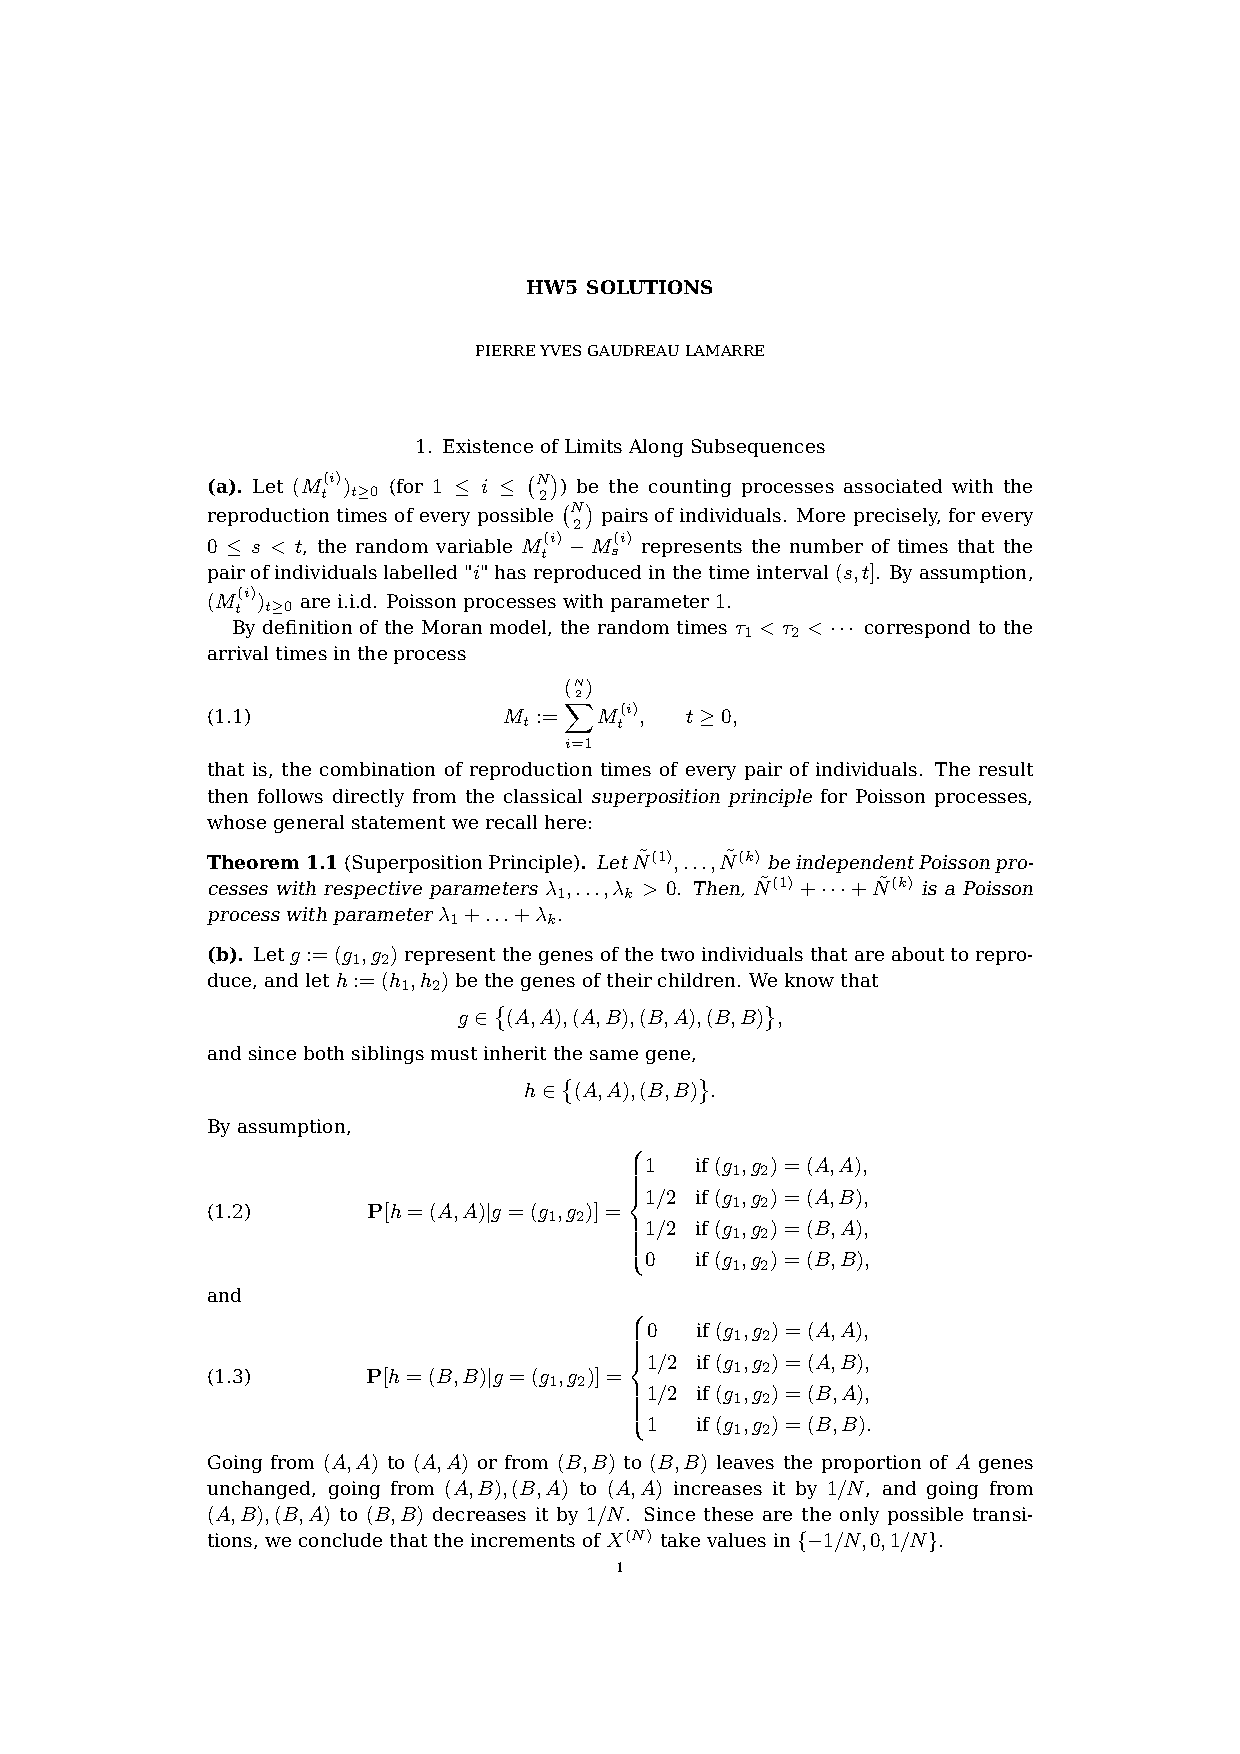
\includepdf[pages=-]{Moran_sol.pdf}

\section{Linkage Between SDE and PDE}
Now, we build the connection between SDE and PDE through the martingale problem.

\subsection{Cauchy Problem}

\begin{definition} \textcolor{red}{(Cauchy Problem)}

The Cauchy problem refers to the following PDE

\begin{equation*}
\partial_tu(t,x)=(\mathcal{A}u)(t,x), \quad t\geq0, x\in\mathbb{R},u(0,x)=g(x)
\end{equation*}
where

\begin{equation*} 
(\mathcal{A}u)(t,x):=b(t,x)\partial_xu(x)+\frac{1}{2}\sigma^2(x)\partial^2_{xx}u(x).
\end{equation*}

\end{definition}

\begin{theorem}
If the above Cauchy problem has a classical solution $u\in C^{1,2}([0,\infty)\times\mathbb{R},\mathbb{R})$ for every function $g\in C_c^\infty(\mathbb{R})$. then weak uniqueness holds for the time-homogeneous SDE

\begin{equation} \label{time_homo_sde}
dX_t=b(X_t)dt + \sigma(X_t)dW_t.
\end{equation}

\end{theorem}

\begin{proof}
Suppose $X$ and $\tilde{X}$ are two weak solutions to the SDE \eqref{time_homo_sde}. First, we aim to show that for each $t\geq0$, $X_t$ and $\tilde{X}_t$ have the same distribution. Define $w(s,x):=u(t-s,x)$, where $u$ is the solution to the Cauchy problem. Then, $w$ satisfies the following PDE:

\begin{equation} \label{cauchy_pf_1}
\partial_s w(s,x)+(\mathcal{A}w)(s,x)=0, \quad s,x\in[0,t]\times\mathbb{R}.
\end{equation}
Applying Ito's formula to $w(t,X-t)$, we get

\begin{equation*}
\begin{aligned}
w(t,X_t)&=w(0,X_0)+\int^t_0\partial_sw(s,X_s)ds + \int^t_0\partial_xw(s,X_s)dX_s+\frac{1}{2}\int^t_0\sigma^2(X_s)\partial^2_{xx}w(s,X_s)ds\\
&=w(0,X_0)+\int^t_0\partial_sw(s,X_s)ds + \int^t_0\partial_xw(s,X_s)b(X_s)ds+\int^t_0\partial_xw(s,X_s)\sigma(X_s)dW_s\\
&\quad+\frac{1}{2}\int^t_0\sigma^2(X_s)\partial^2_{xx}w(s,X_s)ds\\
&=w(0,X_0)+\int^t_0\left(\partial_sw(s,X_s) + (\mathcal{A}w)(s,X_s)\right)ds+\int^t_0\partial_xw(s,X_s)\sigma(X_s)dW_s\\
&=w(0,X_0)+\int^t_0\partial_xw(s,X_s)\sigma(X_s)dW_s,
\end{aligned}
\end{equation*}
where the stochastic integral is a local martingale. Using localization argument and taking expectation, we have

\begin{equation*}
\mathbb{E}[w(t,X_t)]=\mathbb{E}[w(0,X_0)].
\end{equation*}
Using the given initial condition, we get
\begin{equation*}
\mathbb{E}[g(X_t)]=\mathbb{E}[w(0,x)].
\end{equation*}
Same process can be equally applied to the other solution $\tilde{X}_t$, and we obtain $\mathbb{E}[g(X_t)]=\mathbb{E}[g(\tilde{X}_t)]=\mathbb{E}[w(0,x)]$. It implies that $X_t$ and $\tilde{X}_t$ have the same distribution.

Next, we show that for all $n\in\mathbb{N}^*$ and any sequence $0\leq t_1<t_2<...<t_n$, the following is true:

\begin{equation} \label{cauchy_pf_2}
(X_{t_1},X_{t_2},...,X_{t_n})\eqd(\tilde{X}_{t_1},\tilde{X}_{t_2},...,\tilde{X}_{t_n}).
\end{equation}
We use induction. For $n=1$, it is apparent from the result we just showed. Assume \eqref{cauchy_pf_2} holds for some $n\geq1$, and denote by $\mu_n$ the associated probability measure. Consider two measurable set $A\subset\mathbb{R}^n$ and $\tilde{A}\subset\mathbb{R}$, we have

\begin{equation*}
\mathbb{P}((X_{t_1},X_{t_2},...,X_{t_n})\in A\times\tilde{A})=\int_A\mathbb{P}(X_{t_{n+1}}\in\tilde{A}|(X_{t_1},X_{t_2},...,X_{t_n})=x)\mu_n(dx).
\end{equation*}
Thus, if we can show the following holds, then we are done.

\begin{equation*}
\mathbb{P}(X_{t_{n+1}}\in\tilde{A}|(X_{t_1},X_{t_2},...,X_{t_n})=x)=\mathbb{P}(\tilde{X}_{t_{n+1}}\in\tilde{A}|(\tilde{X}_{t_1},\tilde{X}_{t_2},...,\tilde{X}_{t_n})=x)
\end{equation*}
This identity can be shown in the same way as we did in the first step, except for changing the initial condition to $X_{t_n}$. 

\end{proof}

\subsection{Feynman-Kac Representation} \label{sec:feynman-kac}

Next, we discuss another link between the SDE and the PDE, namely the famous Feynman-Kac representation. Loosely speaking, it connects the expected reward from the solution of a SDE to a PDE. Consider the following SDE

\begin{equation} \label{feynman_kac_sde}
dX_s = b(s,X_s)ds + \sigma(s,X_s)dW_s, \quad s\geq t,
\end{equation}
where $(t,x)\in[0,T]\times\mathbb{R}$, $X^{t,x}$ is the strong solution, and $x\in\mathbb{R}$ is the initial condition. The Feynman-Kac formula allows us to establish a link between the following expected reward

\begin{equation} \label{feynman_kac_reward}
v(t,x):=\mathbb{E}\left[e^{\int_t^Tk(u,X_u^{t,x})du}g(X_T^{t,x})+\int^T_te^{-\int^s_tk(u,X_u^{t,x})du}f(s,X_s^{t,x})ds\right],
\end{equation}
and the solution of the following PDE on $(t,x)\in[0,T]\times\mathbb{R}$

\begin{equation} \label{feynman_kac_pde}
k(t,x)w(t,x)-\mathcal{L}w(t,x)-f(t,x)=0, \quad w(T,x)=g(x),
\end{equation}
where $\mathcal{L}$ is the generator of $(t,X_t)$

\begin{equation} \label{feynman_kac_generator}
\mathcal{L}\psi(t,x):=\partial_t\psi(t,x)+\partial_x\psi(t,x)b(t,x)+\frac{1}{2}\partial^2_{xx}\psi(t,x)\sigma^2(t,x),
\end{equation}
for all $\psi(t,x)\in C^{1,2}([0,T]\times\mathbb{R})$.

We assume that the functions $f,g,k,b,\sigma$ are continuous, $k$ is bounded from below by a finite constant \underline{$k$}, and both $f$ and $g$ have polynomial growth. Given that these assumptions hold, we can link \eqref{feynman_kac_reward} and \eqref{feynman_kac_pde} in two directions by the following two Propositions. 

\begin{prop} \label{prop:pde_imply_reward}
Let $w\in C^0([0,T]\times\mathbb{R})\cap C^{1,2}([0,T],\mathbb{R})$ with polynomial growth be a continuous solution to the PDE \eqref{feynman_kac_pde}, then $w=v$ for $v$ defined in \eqref{feynman_kac_reward}.
\end{prop}

\begin{proof}
Fix $(t,x)\in[0,T]\times\mathbb{R}$ and denote $X^{t,x}$ to be the solution to the SDE \eqref{feynman_kac_sde} starting from $x\in\mathbb{R}$ at time $t\in[0,T]$. We will apply Ito's formula between time $t$ and some well-chosen stopping time $\tau_n$ to the following:

\begin{equation} \label{feynman_kac_ito}
\mathcal{K}_{t,x}(s)w(s,X_s^{t,x}), \quad \text{where} \quad \mathcal{K}_{t,x}(s):=e^{-\int^s_tk(u,X_u^{t,x})du}.
\end{equation}
First, applying Ito's formula to $w(s,X_s^{t,x})$, we have

\begin{equation*}
\begin{aligned}
dw(s,X_s^{t,x})&=\partial_sw(s,X_s^{t,x})ds+\partial_xw(s,X_s^{t,x})dX_s^{t,x}+\frac{1}{2}\partial^2_{xx}w(s,X_s^{t,x})d\langle X^{t,x}\rangle_s\\
&=(\mathcal{L}w)(s,X_s^{t,x})ds+\partial_xw(s,X_s^{t,x})\sigma(s,X_s^{t,x})dW_s,
\end{aligned}
\end{equation*}
using the definition of the generator \eqref{feynman_kac_generator}. Then, applying Ito's formula to \eqref{feynman_kac_ito}, we have 

\begin{equation*}
\begin{aligned}
d(K_{t,x}(s)w(s,X_s^{t,x}))&=d\mathcal{K}_{t,x}(s)w(s,X_s^{t,x})+\mathcal{K}_{t,x}(s)d(w(s,X_s^{t,x}))+d\langle w,K\rangle_s\\
&=\mathcal{K}_{t,x}(s)(-k(s,X_s^{t,x})w(s,X_s^{t,x})+(\mathcal{L}w)(s,X_s^{t,x})ds+\partial_xw(s,X_s^{t,x})\sigma(s,X_s^{t,x})dW_s)\\
&=\mathcal{K}_{t,x}(s)(-f(s,X_s^{t,x})+\partial_xw(s,X_s^{t,x})\sigma(s,X_s^{t,x})dW_s),
\end{aligned}
\end{equation*}
where the last identity follows because $w$ is a solution to the PDE \eqref{feynman_kac_pde}. Then, we may write it in the integral form as follows

\begin{equation*}
\begin{aligned}
w(\tau_n,X_{\tau_n}^{t,x})\mathcal{K}_{t,x}(\tau_n)=w(t,x)-\int_t^{\tau_n}\mathcal{K}_{t,x}(s)f(s,X_s^{t,x})+\int_t^{\tau_n}\partial_xw(s,X_s^{t,x})\sigma(s,X_s^{t,x})dW_s,
\end{aligned}
\end{equation*}
where we used the fact that $K_{t,x}(t)=1$, and $\tau_n$ is a stopping time to be define later. Taking expectations on both side, we have

\begin{equation*}
\begin{aligned}
w(t,x)=\mathbb{E}\left[w(\tau_n,X_{\tau_n}^{t,x})\mathcal{K}_{t,x}(\tau_n)+\int_t^{\tau_n}\mathcal{K}_{t,x}(s)f(s,X_s^{t,x})-\int_t^{\tau_n}\partial_xw(s,X_s^{t,x})\sigma(s,X_s^{t,x})dW_s\right].
\end{aligned}
\end{equation*}
Now, comparing this to the desired form in \eqref{feynman_kac_reward}, it remains to properly define the stopping time $\tau_n$ such that $\tau_n\rightarrow T$ as $n\rightarrow\infty$, and the integrand in the stochastic integral is bounded. Let's define the stopping time as

\begin{equation*}
\tau_n:=(T-\frac{1}{n})\wedge \inf \{s\geq t:|X_s^{t,x}|\geq n\}.
\end{equation*}
Through this definition, $|X_s^{t,x}|$ is bounded, and thus the integrand in the stochastic integral is bounded because of the smoothness of$w$ and continuity of $\sigma$. On the other hand, we have $\tau_n\rightarrow T$. By the dominated convergence theorem (using polynomial growth of $f,w$), we have

\begin{equation*}
\begin{aligned}
w(t,x)=\lim_{n\rightarrow\infty}w(t,x)&=\lim_{n\rightarrow\infty}\mathbb{E}\left[w(\tau_n,X_{\tau_n}^{t,x})\mathcal{K}_{t,x}(\tau_n)+\int_t^{\tau_n}\mathcal{K}_{t,x}(s)f(s,X_s^{t,x})\right]\\
&=\mathbb{E}\left[w(T,X_{T}^{t,x})\mathcal{K}_{t,x}(T)+\int_t^{T}\mathcal{K}_{t,x}(s)f(s,X_s^{t,x})\right]\\
&=\mathbb{E}\left[e^{\int_t^Tk(u,X_u^{t,x})du}g(X_T^{t,x})+\int^T_te^{-\int^s_tk(u,X_u^{t,x})du}f(s,X_s^{t,x})ds\right].
\end{aligned}
\end{equation*}
The proof is complete.
\end{proof}

Before showing the converse of the preceding result, the following result is necessary. 

\begin{theorem} \label{thm:dp} \textcolor{red}{(Dynamic Programming Principle)}

Let $\tau$ be a stopping time taking values in $[t,T]$, and $v$ satisfying the expected reward equation \eqref{feynman_kac_reward}. Then:

\begin{equation}
v(t,x)=\mathbb{E}\left[\mathcal{K}_{t,x}(\tau)v(\tau,X_\tau^{t,x})+\int^\tau_t\mathcal{K}_{t,x}(s)f(s,X_s^{t,x})ds\right],
\end{equation}

\end{theorem}

\begin{proof}
From the tower rule, we have

\begin{equation} \label{dp_1}
\begin{aligned}
v(t,x)&=\mathbb{E}\left[e^{\int_t^Tk(u,X_u^{t,x})du}g(X_T^{t,x})+\int^T_te^{-\int^s_tk(u,X_u^{t,x})du}f(s,X_s^{t,x})ds\right]\\
&=\mathbb{E}\left[\mathcal{K}_{t,x}(T)g(X_T^{t,x})+\int^T_t\mathcal{K}_{t,x}(s)f(s,X_s^{t,x})ds\right]\\
&=\left.\mathbb{E}\left[\mathbb{E}\left[\mathcal{K}_{t,x}(T)g(X_T^{t,x})+\int^T_t\mathcal{K}_{t,x}(s)f(s,X_s^{t,x})ds\right\vert\mathcal{F}_\tau\right]\right]\\
&=\mathbb{E}\left[\int^\tau_t\mathcal{K}_{t,x}(s)f(s,X_s^{t,x})ds+\left.\mathbb{E}\left[\mathcal{K}_{t,x}(T)g(X_T^{t,x})\right\vert\mathcal{F}_\tau\right]+\left.\mathbb{E}\left[\int^T_\tau \mathcal{K}_{t,x}(s)f(s,X_s^{t,x})ds\right\vert\mathcal{F}_\tau\right]\right].
\end{aligned}
\end{equation}
In addition, by definition of $K$, for all $s\geq \tau$, we have

\begin{equation*}
\mathcal{K}_{t,x}(s):=e^{-\int^s_tk(u,X_u^{t,x})du}=e^{-\int^\tau_tk(u,X_u^{t,x})du}e^{-\int^s_\tau k(u,X_u^{t,x})du}=\mathcal{K}_{t,x}(\tau)\mathcal{K}_{\tau,X_\tau^{t,x}}(s).
\end{equation*}
Continuing from \eqref{dp_1}, we have

\begin{equation*}
\begin{aligned}
v(t,x)&=\mathbb{E}\left[\int^\tau_t\mathcal{K}_{t,x}(s)f(s,X_s^{t,x})ds+K_{t,x}(\tau)\left.\mathbb{E}\left[\mathcal{K}_{\tau,X_\tau^{t,x}}(T)g(X_T^{t,x})+\int^T_\tau K_{\tau,X_\tau^{t,x}}(s)f(s,X_s^{t,x})ds\right\vert\mathcal{F}_\tau\right]\right]\\
&=\mathbb{E}\left[\int^\tau_t\mathcal{K}_{t,x}(s)f(s,X_s^{t,x})ds+\mathcal{K}_{t,x}(\tau)\left.\mathbb{E}\left[\mathcal{K}_{\tau,y}(T)g(X_T^{\tau,y})+\int^T_\tau \mathcal{K}_{\tau,y}(s)f(s,X_s^{\tau,y})ds\right\vert\mathcal{F}_\tau\right]\right]\\
&=\mathbb{E}\left[\int^\tau_t\mathcal{K}_{t,x}(s)f(s,X_s^{t,x})ds+\mathcal{K}_{t,x}(\tau)\mathbb{E}\left[\mathcal{K}_{\tau,y}(T)g(X_T^{\tau,y})+\int^T_\tau \mathcal{K}_{\tau,y}(s)f(s,X_s^{\tau,y})ds\right]\right]\\
&=\mathbb{E}\left[\mathcal{K}_{t,x}(\tau)v(\tau,X_\tau^{t,x})+\int^\tau_t\mathcal{K}_{t,x}(s)f(s,X_s^{t,x})ds\right],
\end{aligned}
\end{equation*}
where we used $y:=X_\tau^{t,x}$ and, by pathwise uniqueness, $X_s^{t,x}=X_\tau^{t,y}$. The proof is complete.
\end{proof}

Now, we show the converse of Proposition \ref{prop:pde_imply_reward}.

\begin{prop}
If $v$, defined by the expected reward in \eqref{feynman_kac_reward}, is $C^{1,2}([0,T],\mathbb{R})$, then $v$ is the solution to the PDE \eqref{feynman_kac_pde}.
\end{prop}

\begin{proof}
The proof is very similar to the proof for Proposition \ref{prop:pde_imply_reward}. We would like to apply Ito's formula to 

\begin{equation*}
\mathcal{K}_{t,x}(s)v(s,X_s^{t,x}),
\end{equation*}
where $K_{t,x}(s)$ in the same way as \eqref{feynman_kac_ito}. With exactly the same step, we obtain the following

\begin{equation*}
\begin{aligned}
d(K_{t,x}(s)v(s,X_s^{t,x}))=\mathcal{K}_{t,x}(s)(-k(s,X_s^{t,x})v(s,X_s^{t,x})+(\mathcal{L}v)(s,X_s^{t,x})ds+\partial_xv(s,X_s^{t,x})\sigma(s,X_s^{t,x})dW_s).
\end{aligned}
\end{equation*}
In the integral form, we have

\begin{equation*}
\begin{aligned}
v(t,x)=v(\tau,X_\tau^{t,x})\mathcal{K}_{t,x}(\tau)-\int_t^\tau \mathcal{K}_{t,x}(s)(-k(s,X_s^{t,x})v(s,X_s^{t,x})+(\mathcal{L}v)(s,X_s^{t,x}))ds-\int^\tau_t \partial_xv(s,X_s^{t,x})\sigma(s,X_s^{t,x})dW_s.
\end{aligned}
\end{equation*}
Taking expectations, we get

\begin{equation*}
\begin{aligned}
v(t,x)=\mathbb{E}\left[v(\tau,X_\tau^{t,x})\mathcal{K}_{t,x}(\tau)-\int_t^\tau \mathcal{K}_{t,x}(s)(-k(s,X_s^{t,x})v(s,X_s^{t,x})+(\mathcal{L}v)(s,X_s^{t,x}))ds\right]-\mathbb{E}\left[\int^\tau_t \partial_xv(s,X_s^{t,x})\sigma(s,X_s^{t,x})dW_s\right].
\end{aligned}
\end{equation*}
Based on the dynamic programming principle from Theorem \ref{thm:dp}, we have 

\begin{equation*}
0=\mathbb{E}\left[\int^\tau_t\mathcal{K}_{t,x}(s)(kv-\mathcal{L}v-f)(s,X_s^{t,x})\right]-\mathbb{E}\left[\int^\tau_t\mathcal{K}_{t,x}(s)\partial_xv(s,X_s^{t,x})\sigma(s,X_s^{t,x})dW_s\right]
\end{equation*}
Then, we would like to define the stopping time $\tau$ so that it is close to $t$ at some point, which makes the expectation of the stochastic integral vanish. Define

\begin{equation*}
\tau:=(t+h)\wedge\inf\{s\geq t: |X_s^{t,x}-x|\geq 1\}.
\end{equation*}
The integrand of the stochastic integral is bounded, and we can take $h$ to be small enough, so that 

\begin{equation*}
0=\mathbb{E}\left[\frac{1}{h}\int^{t+h}_tK_{t,x}(s)(kv-\mathcal{L}v-f)(s,X_s^{t,x})ds\right]
\end{equation*}
Since the integrand is continuous in time, we have the following convergence result
\begin{equation*}
\lim_{h\rightarrow0}\frac{1}{h}\int^{t+h}_t\mathcal{K}_{t,x}(s)(kv-\mathcal{L}v-f)(s,X_s^{t,x})ds=(kv-\mathcal{L}v-f)(t,x)
\end{equation*}
By the dominated convergence theorem, we have
\begin{equation*}
(kv-\mathcal{L}v-f)(t,x)=\lim_{h\rightarrow0}\mathbb{E}\left[\frac{1}{h}\int^{t+h}_t\mathcal{K}_{t,x}(s)(kv-\mathcal{L}v-f)(s,X_s^{t,x})ds\right]=0
\end{equation*}
The proof is complete.
\end{proof}

\section{Stochastic Optimal Control}
In this section, we introduce the stochastic optimal control problem. In this regime, an agent controls a system, which evolves under a SDE, to optimize a given criterion. In particular, it is formulated with the following three features: the system state, the control, and the performance/cost criterion. 

\subsection{Finite Horizon Problem}
As an initial step, we formulate the stochastic optimal control problem in a finite time horizon, i.e., $t\in[0.T]$, where $T<\infty$. Moreover, we work on a fixed probability space $(\Omega,\mathcal{F}, \mathbb{F}, \mathbb{P})$, satisfying the usual condition and carrying a one-dimensional Brownian motion $W$.  

We first define the set of admissible controls as follows:

\begin{equation*}
\mathcal{A}:=\biggl\{\alpha\in A: \mathbb{F}-\text{progressively measurable, and }\mathbb{E}\left[\int^T_0|\alpha_s|^2ds\right]<\infty\biggl\},
\end{equation*}
for some $A\in\mathbb{R}$. Then, we require the system state evolves under the following controlled SDE

\begin{equation} \label{sde_control}
dX_t = b(t,X_t,\alpha_t)dt + \sigma_t(X_t,\alpha_t)dW_t,
\end{equation}
where $\alpha_t$ is the admissible control, i.e., $\alpha_t\in\mathcal{A}$. To guarantee the existence (and uniqueness) of such a state, we impose the following assumptions on the function $b$ and $\sigma$

\begin{equation} \label{SOC_assumption}
\begin{aligned}
&|b(t,x,\alpha)-b(t,y,\alpha)|+|\sigma(t,x,\alpha)-\sigma(t,y,\alpha)|\leq K(|x-y|)\\
&|b(t,x,\alpha)+\sigma(t,x,\alpha)|\leq K(1+|x|+|\alpha|),
\end{aligned}
\end{equation}
for some constant $K\in\mathbb{R}$. Then, the following results follow directly from Theorem \eqref{thm:strong_existence} and \eqref{thm:strong_uniqueness}.

\begin{prop}
Under assumptions \eqref{SOC_assumption}, we have that for all initial conditions $(t,x)\in[0,T]\times\mathbb{R}$ and all control processes $\alpha\in\mathcal{A}$, there exists a unique strong solution $X^{t,x,\alpha}$ to the SDE \eqref{sde_control}. Moreover, for every $T>0$, there exists a constant $C>0$ such that:

\begin{equation*}
\mathbb{E}\left[\sup_{t\leq s\leq T}|X_s^{t,x,\alpha}|^2\right]\leq C(1+|x|^2)e^{Ct}, \quad \forall t\in[0,T].
\end{equation*}
\end{prop}

The objective of the control problem (in other words, the condition under which we choose the control process $\alpha\in\mathcal{A}$) is described by the following functional $J$. 

\begin{equation*}
J(t,x,\alpha):=\mathbb{E}\left[\mathcal{K}_{t,x,\alpha}(T)g(X_T)+\int^T_t\mathcal{K}_{t,x,\alpha}(s)f(s,X_s,\alpha_s)ds\right],
\end{equation*}
where $g:\mathbb{R}\rightarrow\mathbb{R}$ is the final reward, $f:[0,T]\times\mathbb{R}\times A\rightarrow\mathbb{R}$ is the running reward, and 
\begin{equation} \label{def_k}
\mathcal{K}_{t,x,\alpha}(s):=\exp(-\int^s_tk(u,X_u,\alpha_u)du),
\end{equation}
where $k:[0,T]\times\mathbb{R}\times A\rightarrow\mathbb{R}$ is the discount factor. We further impose the following assumptions to the reward functional:

\begin{equation*}
|f(t,x,\alpha)|+|g(x)|\leq K(1+|\alpha|+|x|^2), \quad \forall (t,x,\alpha)\in[0,T)\times\mathbb{R}\times A.
\end{equation*}
Finally, the value function starting at $(t,x)\in[0,T]\times\mathbb{R}$ is defined as the maximum of $J$ over admissible controls $\alpha\in\mathcal{A}$:

\begin{equation*} 
V(t,x):=\sup_{\alpha\in\mathcal{A}}J(t,x,\alpha).
\end{equation*}

In summary, the finite-time stochastic optimal control problem is formulated as follows

\begin{definition} \textcolor{red}{(Finite-Time Stochastic Optimal Control Problem)}
Let $(t,x)\in]0,T]\times\mathbb{R}$ be the initial condition, we consider the following stochastic optimal control problem
\begin{equation} \label{soc:value_fcn}
V(t,x):=\sup_{\alpha\in\mathcal{A}}J(t,x,\alpha),
\end{equation}
where the performance criterion $J$ is defined, for $\alpha\in\mathcal{A}$, by

\begin{equation} \label{soc:cost_fcn}
J(t,x,\alpha):=\mathbb{E}\left[\mathcal{K}_{t,x,\alpha}(T)g(X_T)+\int^T_t\mathcal{K}_{t,x,\alpha}(s)f(s,X_s,\alpha_s)ds\right],
\end{equation}
where the state of the system $X^{t,x,\alpha}$ satisfies $X_t=x$ and is solution to the following SDE:

\begin{equation} \label{sde_control}
dX_s = b(s,X_s,\alpha_s)ds + \sigma_s(X_s,\alpha_s)dW_s, \quad s\in[t,T].
\end{equation}
Solving this problem consists of computing the value function and determining the optimal control $\alpha^*\in\mathcal{A}$ such that $V(t,x):=J(t,x,\alpha^*)$. 
\end{definition}

We first state the dynamic programming principle for the stochastic optimal control problem, the counterpart of Theorem \ref{thm:dp}. It is a consequence of the Markov property of the dynamics. Intuitively, solving the problem between time $t$ and $T$ is equivalent to:

\begin{enumerate}
\item
Solving the problem between some time $s\in[t,T]$ and $T$, i.e., computing the value function $V(s,X_s)$ and the associated optimal control $(\alpha^*_u)_{u\in[s,T]}$.

\item
Solving the problem between $t$ and $s$, where the terminal value at time $s$ is given by the value computed at the previous step. 
\end{enumerate}

Formally speaking, we have

\begin{theorem} \label{thm:dp_hjb}
Let $(t,x)\in[0,T]\times\mathbb{R}$. For any $[t,T]$-valued stopping time $\tau$, we have:

\begin{equation*}
V(t,x)=\sup_{\alpha\in\mathcal{A}_t}\mathbb{E}\left[\mathcal{K}_{t,x,\alpha}(\tau)V(\tau,X_\tau^{t,x,\alpha})+\int^\tau_t\mathcal{K}_{t,x,\alpha}(s)f(s,X_s^{t,x,\alpha},\alpha_s)ds\right].
\end{equation*}
\end{theorem}

\begin{proof}
Following the same steps in the proof of Theorem \ref{thm:dp}, we have the following:

\begin{equation*}
J(t,x,\alpha)=\mathbb{E}\left[\mathcal{K}_{t,x,\alpha}(\tau)J(\tau,X_\tau^{t,x,\alpha},\alpha)+\int^\tau_t\mathcal{K}_{t,x,\alpha}(s)f(s,X_s^{t,x,\alpha},\alpha_s)ds\right].
\end{equation*}
By the definition of the value function, we know that $J(s,y,\alpha)\leq V(s,y)$ for all $(s,y)\in[t,T]\times\mathbb{R}$ and $\alpha\in\mathcal{A}_t$. It then implies

\begin{equation*}
\mathbb{E}\left[\mathcal{K}_{t,x,\alpha}(\tau)J(\tau,X_\tau^{t,x,\alpha},\alpha)+\int^\tau_t\mathcal{K}_{t,x,\alpha}(s)f(s,X_s^{t,x,\alpha},\alpha_s)ds\right]\leq \mathbb{E}\left[\mathcal{K}_{t,x,\alpha}(\tau)V(\tau,X_\tau^{t,x,\alpha})+\int^\tau_t\mathcal{K}_{t,x,\alpha}(s)f(s,X_s^{t,x,\alpha},\alpha_s)ds\right].
\end{equation*}
Then, taking the supremum, we have

\begin{equation*}
V(t,x)=\sup_{\alpha\in\mathcal{A}_t}J(t,x,\alpha)\leq \sup_{\alpha\in\mathcal{A}_t}\mathbb{E}\left[\mathcal{K}_{t,x,\alpha}(\tau)V(\tau,X_\tau^{t,x,\alpha})+\int^\tau_t\mathcal{K}_{t,x,\alpha}(s)f(s,X_s^{t,x,\alpha},\alpha_s)ds\right].
\end{equation*}

Next, we need to the show the converse. By definition, $V(\tau,X_\tau^{t,x},\alpha)$ is the optimal performance over all admissible control, $\alpha\in\mathcal{A}_t$, starting at $\tau$. Then, for any $\epsilon>0$, there must be an $\epsilon$-optimal control  $\alpha^\epsilon\in\mathcal{A}_\tau$, such that 

\begin{equation*}
V(\tau,y)-\epsilon\leq J(\tau,y,\alpha^\epsilon), \quad \forall y\in\mathbb{R}
\end{equation*}

Then, we may define the control process 

\begin{equation*}
\hat{\alpha}_s:=
\begin{cases}
\alpha_s, & \text{if } x\in[t,\tau]\\
\alpha^\epsilon_s, & \text{if } x\in[\tau,T]
\end{cases}
\end{equation*}
It can be shown that the process $\hat{\alpha}$ defined above is progressively measurable, and there fore that $\hat{\alpha}\in\mathcal{A}$. However, the proof of this point involves delicate measurability arguments, namely the measurable selection theorem. We shall not address this issue and take $\hat{\alpha}\in\mathcal{A}$ for granted. By definition, we have

\begin{equation*}
\begin{aligned}
V(\tau,y)&\geq\mathbb{E}\left[\mathcal{K}_{t,x,\hat{\alpha}}(\tau)J(\tau,X_\tau^{t,x,\hat{\alpha}},\alpha^\epsilon)+\int^\tau_t\mathcal{K}_{t,x,\hat{\alpha}}(s)f(s,X_s^{t,x,\hat{\alpha}},\alpha_s)ds\right]\\
&\geq\mathbb{E}\left[\mathcal{K}_{t,x,\hat{\alpha}}(\tau)(V(\tau,X_\tau^{t,x,\hat{\alpha}})-\epsilon)+\int^\tau_t\mathcal{K}_{t,x,\hat{\alpha}}(s)f(s,X_s^{t,x,\hat{\alpha}},\alpha_s)ds\right].
\end{aligned}
\end{equation*}
After taking supremum and letting $\epsilon\rightarrow0$, we have

\begin{equation*}
\begin{aligned}
V(\tau,y)\geq\sup_{\alpha\in\mathcal{A}_t}\mathbb{E}\left[\mathcal{K}_{t,x,\alpha}(\tau)V(\tau,X_\tau^{t,x,\alpha})+\int^\tau_t\mathcal{K}_{t,x,\alpha}(s)f(s,X_s^{t,x,\alpha},\alpha_s)ds\right].
\end{aligned}
\end{equation*}
The proof is complete.
\end{proof}

\subsubsection{The Hamilton-Jacobi-Bellman Equation}

We introduce the Hamiltonian-Jacobi-Bellman (HJB) equation in this part to provide an equivalent way of finding the optimal control and value function in the stochastic optimal control problem. It is closely related to the Feynman-Kac representation discussed in Section \ref{sec:feynman-kac}. The Hamiltonian map $\mathcal{H}: [0,T]\times\mathbb{R}\times\mathbb{R}\times\mathbb{R}\times\mathbb{R}\rightarrow\mathbb{R}$ associated to our optimal control problem is defined as 
    
\begin{equation}
\mathcal{H}(t,x,y,z,\gamma):=\sup_{a\in A}\Big\{-k(t,x,a)y+b(t,x,a)z+\frac{1}{2}\sigma^2(t,x,a)\gamma+f(t,x,a)\Big\}.
\end{equation}
The HJB equation associated to out control problem is the following:

\begin{equation} \label{hjb}
-\partial_tv(t,x)-\mathcal{H}(t,x,v(t,x),\partial_xv(t,x),\partial^2_{xx}v(t,x))=0, \quad (t,x)\in[0,T]\times\mathbb{R},
\end{equation}
with terminal condition $v(T,x)=g(x),x\in\mathbb{R}$. To make connection to the PDE obtained for the Feynman-Kac representation discussed in Section \ref{sec:feynman-kac}, we can define the generator $\mathcal{L}^a$ with constant control $a\in A$ as follows:

\begin{equation}
\mathcal{L}^a\psi(t,x):=\partial_t\psi(t,x)+\partial_x\psi(t,x)b(t,x,a)+\frac{1}{2}\partial^2_{xx}\psi(t,x)\sigma^2(t,x,a), \quad\psi\in C^{1,2}([0,T]\times\mathbb{R}).
\end{equation}
Using this notation, the HJB equation \eqref{hjb} can be written as 

\begin{equation}
-\sup_{a\in A}\{\mathcal{L}^av(t,x)-k(t,x,a)v(t,x)+f(t,x,a)\}=0, \quad (t,x)\in[0,T].
\end{equation}
Comparing this formula to \eqref{feynman_kac_pde}, the only difference is that we have a supremum over admissible control here. To simplify, we often write:

\begin{equation} \label{hjb_simple}
\sup_{a\in A}\{\mathcal{L}^av-k^av+f^a\}=0.
\end{equation}

\begin{theorem} \label{thm:soc_value_imply_hjb}
Assume the value function in \eqref{soc:value_fcn} is smooth, namely $V\in C^{1,2}([0,T]\times\mathbb{R})$, and the map $(t,x)\rightarrow\mathcal{H}(t,x,V(t,x),\partial_xV(t,x),\partial^2_{xx}V(t,x)$ is continuous. Then, $V$ is solution to the HJB equation \eqref{hjb}.
\end{theorem}

\begin{proof}
First, we check that $V$ satisfies the terminal condition by the following:

\begin{equation*}
V(T,x)=\sup_{\alpha\in\mathcal{A}_t}\mathbb{E}[g(X_T^{T,x,a})]=g(x), \quad x\in\mathbb{R}.
\end{equation*}

As demonstrated above, the HJB equation \eqref{hjb} is equivalent to \eqref{hjb_simple}. We first show $-\{\mathcal{L}^aV+k^aV-f^a\}\geq0$ for all $a\in A$. Let $a\in A$ and consider the constant control $\alpha\in\mathcal{A}$ defined by $\alpha_s=a$ for all $s\in[0,T]$. With $X$ being the solution to the SDE \eqref{sde_control} with constant control $\alpha$, we apply Ito's formula to $V(s,X_s)$ and get

\begin{equation*}
\begin{aligned}
dV(t,X_t)&=\partial_tV(t,X_t)dt + \partial_xV(t,X_t)dX_t + \frac{1}{2}\partial^2_{xx}V(t,X_t)\sigma^2(t,x,a)dt\\
&=(\mathcal{L}^aV)(t,X_t)dt + \partial_xV(t,X_t)\sigma(t,X_t,a)dW_t.
\end{aligned}
\end{equation*}
Then, we apply product rule to $d(V(s,X_s)\mathcal{K}_{t,x,\alpha}(s))$ as follows

\begin{equation*}
\begin{aligned}
d(V(s,X_s)\mathcal{K}_{t,x,a}(s))&=\mathcal{K}_{t,x,a}(s)dV(s,X_s)+V(s,X_s)d\mathcal{K}_{t,x,a}(s)\\
&=\mathcal{K}_{t,x,a}(s)dV(s,X_s)-V(s,X_s)k(s,X_s.a)\mathcal{K}_{t,x,a}(s),
\end{aligned}
\end{equation*}
by the definition of $\mathcal{K}$ in \eqref{def_k}. Combining these two equations and integrating between $t$ and some stopping time $\tau$, we get

\begin{equation*}
\begin{aligned}
V(\tau,X_\tau)\mathcal{K}_{t,x,a}(\tau)&=V(t,x)+\int^\tau_t\mathcal{K}_{t,x,a}(s)[\mathcal{L}^aV-\mathcal{K}^aV](s,X_s)ds+\frac{1}{2}\int^\tau_t\mathcal{K}_{t,x,a}(s)\partial_xV(s,X_s)\sigma(s,X_s,a)dW_s.
\end{aligned}
\end{equation*}
Now we aim to define the stopping time $\tau$ so that the stochastic integral becomes a martingale and $\tau\rightarrow t$.

\begin{equation} \label{stp_time_hjb}
\begin{aligned}
\tau:=(t+h)\wedge\inf\{s\geq t:|X_s-x|\geq1\}.
\end{aligned}
\end{equation}
Because of the continuity of $\sigma$ and $V$, the integrand in the stochastic integral is bounded. Taking expectations, we have

\begin{equation*}
\begin{aligned}
V(t,x)=\mathbb{E}\left[V(\tau,X_\tau)\mathcal{K}_{t,x,a}(\tau)+\int^\tau_t\mathcal{K}_{t,x,a}(s)[k^aV-\mathcal{L}^aV](s,X_s)ds\right].
\end{aligned}
\end{equation*}
Using the dynamic programming results in Theorem \ref{thm:dp_hjb}, we have 

\begin{equation*}
\begin{aligned}
V(t,x)&=\mathbb{E}\left[V(\tau,X_\tau)\mathcal{K}_{t,x,a}(\tau)+\int^\tau_t\mathcal{K}_{t,x,a}(s)[k^aV-\mathcal{L}^aV](s,X_s)ds\right]\\
&\geq\mathbb{E}\left[\mathcal{K}_{t,x,\alpha}(\tau)V(\tau,X_\tau^{t,x,\alpha})+\int^\tau_t\mathcal{K}_{t,x,\alpha}(s)f(s,X_s^{t,x,\alpha},\alpha_s)ds\right],
\end{aligned}
\end{equation*}
which then implies

\begin{equation*}
\begin{aligned}
\mathbb{E}\left[\int^\tau_t\mathcal{K}_{t,x,a}(s)[k^aV-\mathcal{L}^aV-f^a](s,X_s)ds\right]\geq0.
\end{aligned}
\end{equation*}
As $h$ close to $0$, $\tau\rightarrow t+h$, we have (by the dominated convergence theorem)

\begin{equation*}
\begin{aligned}
\lim_{h\rightarrow0}\frac{1}{h}\mathbb{E}\left[\int^{t+h}_t\mathcal{K}_{t,x,a}(s)[-\mathcal{L}^aV+\mathcal{K}^aV-f^a](s,X_s)ds\right]=[-\mathcal{L}^aV+\mathcal{K}^aV-f^a](t,X_t)\geq0.
\end{aligned}
\end{equation*}
Since this inequality holds for every control $a\in A$, we conclude by 

\begin{equation*}
\begin{aligned}
-\sup_{a\in A}\{[\mathcal{L}^aV-\mathcal{K}^aV+f^a](t,X_t)\}\geq0.
\end{aligned}
\end{equation*}

It remains to prove the other direction, namely $-\partial_tV(t,x)-\mathcal{H}(t,x,V(t,x),\partial_xV(t,x),\partial^2_{xx}V(t,x))\leq0$ for all $(t,X_t)\in[0,T]\times\mathbb{R}$. Assume that there exists $(t_0,X_0)\in[0,T]\times\mathbb{R}$ such that 

\begin{equation*}
\begin{aligned}
-\partial_tV(t_0,X_0)-\mathcal{H}(t_0,X_0,V(t_0,X_0),\partial_xV(t_0,X_0),\partial^2_{xx}V(t_0,X_0))>0.
\end{aligned}
\end{equation*}
Define $\psi(t,x):=V(t,x)+\epsilon((t-t_0)^2+(x-x_0)^4)$, for some $\epsilon>0$. Then, we know $\psi(t,x)\geq V(t,x)$ with equality holds only when $(t,x)=(t_0,x_0)$. We also have

\begin{equation*}
\begin{aligned}
-\partial_t\psi(t_0,X_0)-\mathcal{H}(t_0,X_0,\psi(t_0,X_0),\partial_x\psi(t_0,X_0),\partial^2_{xx}\psi(t_0,X_0))>0.
\end{aligned}
\end{equation*}
By continuity of the Hamiltonian $\mathcal{H}$, we may define $N_r:=(t_0-r,t_0+r)\times(X_0-r,X_0+r)$ such that 

\begin{equation*}
\begin{aligned}
h(t,X_t)&:=\partial_t\psi(t,X_t)+\mathcal{H}(t,X_t,\psi(t,X_t),\partial_x\psi(t,X_t),\partial^2_{xx}\psi(t,X_t))\\
&=\sup_{a\in A}\{[\mathcal{L}^a\psi-\mathcal{K}^a\psi+f^a](t,X_t)\}\\
&<0,
\end{aligned}
\end{equation*}
for all $(t,X_t)\in N_r$. Next, we define the stopping time

\begin{equation*}
\begin{aligned}
\tau^\alpha:=\inf\{t>t_0:(t,X_t^{t_0,x_0,\alpha})\notin N_r\}.
\end{aligned}
\end{equation*}
By pathwise continuity of the controlled process, we know $(\tau^\alpha,X_{\tau^\alpha}^{t_0,x_0,\alpha})\in\delta N_r$. Define $\eta:=-\max_{\delta N_r}(V-\psi)$, then we have

\begin{equation*}
\begin{aligned}
-\eta=\max_{\delta N_r}(V_\psi)\geq(V-\psi)(\tau^\alpha,X_{\tau^\alpha}^{t_0,x_0,\alpha}).
\end{aligned}
\end{equation*}
Now, we apply Ito's formula to $K_{t_0,x_0,\alpha}(t)\psi(t,X_t^{t_0,x_0,\alpha})$ between $t$ and $\tau^\alpha$, and take expectation. With exactly the same process as previous steps, we simplify the intermediate process and notice that the stochastic integral is a martingale by the definition of stopping time $\tau^\alpha$. We have

\begin{equation*}
\begin{aligned}
\psi(t_0,x_0)&=\mathbb{E}\left[\psi(\tau^\alpha,X_{\tau^\alpha}^{t_0,x_0,\alpha})\mathcal{K}_{t_0,x_0,\alpha}(\tau^\alpha)+\int^{\tau^\alpha}_{t_0}\mathcal{K}_{t_0,x_0,\alpha}(s)[k^\alpha\psi-\mathcal{L}^\alpha\psi](t,X_t^{t_0,x_0,\alpha})dt\right]\\
&\geq\mathbb{E}\left[\psi(\tau^\alpha,X_{\tau^\alpha}^{t_0,x_0,\alpha})\mathcal{K}_{t_0,x_0,\alpha}(\tau^\alpha)+\int^{\tau^\alpha}_{t_0}\mathcal{K}_{t_0,x_0,\alpha}(s)[f^\alpha-h](t,X_t^{t_0,x_0,\alpha})dt\right]\\
&\geq\mathbb{E}\left[\psi(\tau^\alpha,X_{\tau^\alpha}^{t_0,x_0,\alpha})\mathcal{K}_{t_0,x_0,\alpha}(\tau^\alpha)+\int^{\tau^\alpha}_{t_0}\mathcal{K}_{t_0,x_0,\alpha}(s)f^\alpha(t,X_t^{t_0,x_0,\alpha})dt\right]\\
&\geq\eta\mathbb{E}[\mathcal{K}_{t_0,x_0,\alpha}(\tau^\alpha)]+\mathbb{E}\left[V(\tau^\alpha,X_{\tau^\alpha}^{t_0,x_0,\alpha})\mathcal{K}_{t_0,x_0,\alpha}(\tau^\alpha)+\int^{\tau^\alpha}_{t_0}\mathcal{K}_{t_0,x_0,\alpha}(s)f^\alpha(t,X_t^{t_0,x_0,\alpha})dt\right]\\
&>\mathbb{E}\left[V(\tau^\alpha,X_{\tau^\alpha}^{t_0,x_0,\alpha})\mathcal{K}_{t_0,x_0,\alpha}(\tau^\alpha)+\int^{\tau^\alpha}_{t_0}\mathcal{K}_{t_0,x_0,\alpha}(s)f^\alpha(t,X_t^{t_0,x_0,\alpha})dt\right]
\end{aligned}
\end{equation*}
Finally, since $V(t_0,x_0)=\psi(t_0,x_0)$, we have

\begin{equation*}
\begin{aligned}
V(t_0,x_0)>\mathbb{E}\left[V(\tau^\alpha,X_{\tau^\alpha}^{t_0,x_0,\alpha})\mathcal{K}_{t_0,x_0,\alpha}(\tau^\alpha)+\int^{\tau^\alpha}_{t_0}\mathcal{K}_{t_0,x_0,\alpha}(s)f^\alpha(t,X_t^{t_0,x_0,\alpha})dt\right],
\end{aligned}
\end{equation*}
which is contradictory to the dynamic programming principle in Theorem \ref{thm:dp_hjb}. Thus, we conclude that we must have $-\sup_{a\in A}\{[\mathcal{L}^aV-\mathcal{K}^aV+f^a](t,X_t)\}\leq0$, for all $(t,x)\in[0,T]\times\mathbb{R}$.

The proof is complete.

\end{proof}

\begin{rk}
The second part of the proof above can be simplified quite a lot if we knew in advance that there exists an optimal control $\alpha^*$. 

From the dynamic programming principle in Theorem \ref{thm:dp_hjb}, we have 

\begin{equation*}
V(t,x)=\mathbb{E}\left[\mathcal{K}_{t,x,\alpha^*}(\tau)V(\tau,X_\tau^{t,x,\alpha^*})+\int^\tau_t\mathcal{K}_{t,x,\alpha^*}(s)f(s,X_s^{t,x,\alpha^*},\alpha^*_s)ds\right].
\end{equation*}
With the exact same definition of the stopping time as in \eqref{stp_time_hjb} and the same processes of applying the Ito's formula, we have

\begin{equation*}
\begin{aligned}
V(t,x)=\mathbb{E}\left[V(\tau,X_\tau)\mathcal{K}_{t,x,\alpha^*}(\tau)+\int^\tau_t\mathcal{K}_{t,x,\alpha^*}(s)[k^{\alpha^*}V-\mathcal{L}^{\alpha^*}V](s,X_s)ds\right].
\end{aligned}
\end{equation*}
Combining these two equations, we have

\begin{equation*}
\begin{aligned}
\mathbb{E}\left[\int^\tau_t\mathcal{K}_{t,x,\alpha^*}(s)[\mathcal{L}^{\alpha^*}V-k^{\alpha^*}V+f^{\alpha^*}](s,X_s)ds\right]=0,
\end{aligned}
\end{equation*}
which implies (by the dominated convergence theorem)

\begin{equation*}
\begin{aligned}
[\mathcal{L}^{\alpha^*}V-k^{\alpha^*}V+f^{\alpha^*}](s,X_s)=0.
\end{aligned}
\end{equation*}
 Then, we may conclude base on the following

\begin{equation*}
\begin{aligned}
-\sup_{\alpha\in A}[\mathcal{L}^{\alpha^*}V-k^{\alpha^*}V+f^{\alpha^*}]\leq-[\mathcal{L}^{\alpha^*}V-k^{\alpha^*}V+f^{\alpha^*}]=0.
\end{aligned}
\end{equation*}

\end{rk}

The verification theorem shows the reverse direction of Theorem \ref{thm:soc_value_imply_hjb}, i.e., if there is a relatively smooth solution to the HJB equation, then it corresponds to the value function. More precisely, we have the following result. 

\begin{theorem}
Let $w(t,x)\in C^0([0,T]\times\mathbb{R})\cap C^{1,2}([0,T]\times\mathbb{R})$ with quadratic growth in $x$. 
\begin{enumerate}
\item
If $w$ is such that $w(T,x)\geq g(x)$ on $\mathbb{R}$ and is a super solution to \eqref{hjb_simple}, i.e.,

\begin{equation} \label{soc:ver}
\sup_{a\in A}\{\mathcal{L}w(t,x)-k^a(t,x)w(t,x)+f^a(t,x)\}\geq0,
\end{equation}
then $w(t,x)\geq V(t,x)$ for $(t,x)\in[0,T]\times\mathbb{R}$, where $V$ is the value function \eqref{soc:value_fcn}.

\item
Assume that there exists a measurable function $\hat{\alpha}:[0,T)\times\mathbb{R}\rightarrow A$ such that for all $(t,x)\in[0,T]\times\mathbb{R}$, the following SDE has a strong solution

\begin{equation}
dX_s=b(s,X_s,\hat{\alpha}(s,X_s))dX_s+\sigma(s,X_s,\hat{\alpha}(s,X_s))dW_s,
\end{equation}
and such that

\begin{equation}
\mathcal{L}^{\hat{\alpha}(t,x)}w(t,x)-k(t,x,\hat{\alpha}(t,x))w(t,x)+f(t,x,\hat{\alpha}(t,x))\geq0.
\end{equation}
Define the process $\alpha^*$ for all $s\in[0,T]$ by $\alpha^*_s:=\hat{\alpha}(s,X_s)$, and assume $\alpha^*_s\in\mathcal{A}$. If in addition, $w$ satisfies $w(T,x)\leq g(x)$, then $w(t,x)\leq J(t,x,\alpha^*)$, with $J(t,x,\alpha^*)$ being defined in \eqref{soc:cost_fcn}.
\end{enumerate}
\end{theorem}

\begin{proof}
Fix $(t,x)\in[0,t]\times\mathbb{R}$ and $\alpha\in\mathcal{A}_t$. We apply Ito's formula to $\mathcal{K}_{t,x,\alpha}w$ between time $t$ and some stopping time $\tau^n$, and obtain

\begin{equation*}
\begin{aligned}
d(\mathcal{K}_{t,x,\alpha}(t)w(t,X_t))&=d\mathcal{K}_{t,x,\alpha}(t)w(t,X_t)+\mathcal{K}_{t,x,\alpha}(t)dw(t,X_t)\\
&=-\mathcal{K}_{t,x,\alpha}(t)k^{\alpha_t}(t,X_t)w(t,X_t)+\mathcal{K}_{t,x,\alpha}(t)[\mathcal{L}^{\alpha_t}w(t,x)+\partial_xw(t,x)\sigma(t,X_t,\alpha_t)dW_t]\\
&=\mathcal{K}_{t,x,\alpha}(t)[-k^{\alpha_t}(t,X_t)w(t,X_t)+\mathcal{L}^{\alpha_t}w(t,x)+\partial_xw(t,x)\sigma(t,X_t,\alpha_t)dW_t].
\end{aligned}
\end{equation*}

It can be written in the integral form as follows:

\begin{equation*}
\begin{aligned}
\mathcal{K}_{t,x,\alpha}(\tau^n)w(\tau^n,X_{\tau^n})=w(t,x)+\int^{\tau^n}_t\mathcal{K}_{t,x,\alpha}(s)&[-k^{\alpha_s}(s,X_s)w(s,X_s)+\mathcal{L}^{\alpha_s}w(s,x)]ds\\
&+\int^{\tau^n}_t\mathcal{K}_{t,x,\alpha}(s)\partial_xw(s,x)\sigma(s,X_s,\alpha_t)dW_s.
\end{aligned}
\end{equation*}

Choosing the stopping time as follows

\begin{equation*}
\begin{aligned}
\tau^n:=(T-\frac{1}{n}) \wedge \inf\{s\geq t:|X_s-x|\geq n\},
\end{aligned}
\end{equation*}
the stochastic integral is a martingale, and we have

\begin{equation*}
\begin{aligned}
\mathbb{E}[w(t,x)]&=\mathbb{E}\left[\mathcal{K}_{t,x,\alpha}(\tau^n)w(\tau^n,X_{\tau^n})-\int^{\tau^n}_t\mathcal{K}_{t,x,\alpha}(s)[-k^{\alpha_s}(s,X_s)w(s,X_s)+\mathcal{L}^{\alpha_s}w(s,x)]ds\right]\\
&\geq\mathbb{E}\left[\mathcal{K}_{t,x,\alpha}(\tau^n)w(\tau^n,X_{\tau^n})+\int^{\tau^n}_t\mathcal{K}_{t,x,\alpha}(s)f(x,X_s,\alpha_s)ds\right].
\end{aligned}
\end{equation*}
By the continuity of $w$, we have

\begin{equation*}
\lim_{n\rightarrow\infty}w(\tau^n,X_{\tau^n})=w(T,X_T)\geq g(X_T).
\end{equation*}
By Fatou's lemma, we obtain

\begin{equation*}
\begin{aligned}
\mathbb{E}[w(t,x)]\geq\mathbb{E}\left[\mathcal{K}_{t,x,\alpha}(T)g(X_T)+\int^{\tau^n}_t\mathcal{K}_{t,x,\alpha}(s)f(x,X_s,\alpha_s)ds\right].
\end{aligned}
\end{equation*}
The results \eqref{soc:ver} directly follows. 

The proof for the second part is omitted, as it is very similar to the proof for the first part. 

\end{proof}

\begin{rk}
In general, this theorem is used by considering the same function $w$ for both parts, so that one obtains $w(t,x)=V(t,x)$ for all $(t,x)\in[0,T]\times\mathbb{R}$ and the optimal control is given by $\alpha^*$.
\end{rk}




\end{document}